\chapter{数理統計学}
データの出現頻度を近似する式である確率密度関数、累積分布関数について説明し、様々な形の確率密度関数について説明する。
さらに、特定の分布に従う確率変数が、その分布関数から生成された確率変数であることを確かめる方法について説明する。
最後に、モデルの確率変数への当てはまりの良さの相対的な指標である尤度を導入し、尤度を最大にする母数を推定する方法を説明する。
さらに、モデルのパラメータの数に対するペナルティを導入した指標のAICを導入する。

\subsection{確率密度関数}

\subsection{累積分布関数}
aaa

\subsection{相補累積分布関数}
$1$から累積度数を引いたものは、相補累積分布関数と呼ばれ、ある値よりも大きな値をえる確率示し、数式では、
\begin{eqnarray}
    1-F(x) &=& f(X>x) \\
        &=& \int_{x}^{\infty} f(z)dz.
\end{eqnarray}
図\ref{fig:standard_normal_distribution}(c)に図示した。累積分布関数と相補累積分布関数のどちらかを表示するかは、分野によって異なる。
生物学の分野などでは、より大きな値を得る確率を重視することがあるので、累積分布関数よりも、相補累積分布関数が好まれることがあるように私は感じている。

\section{確率変数}
\subsection{確率変数がある分布関数に従う}
確率変数$x$が、ある分布関数に従うとは、

$x$をたくさん集めて、$x_1,x_2,\cdots,x_n$という標本を得たときに、その出現頻度がその分布関数に精度よく近似できる。


\section{正規分布}
正規分布の確率密度関数は、
\begin{equation}
p(x;\mu,\sigma)=\frac{1}{\sqrt{2\pi\sigma^2}}\exp\left(-\frac{(x-\mu)^2}{2\sigma^2} \right)
\end{equation}
ここで、$\mu,\sigma^2$は、正規分布のパラメータで、それぞれ母数平均、母数分散です。
母数平均は最も出現頻度の高い数値を表しており、この値を中心にし、対象に分布が広がります。言い換えれば、$\mu-a$と、$\mu+a$の出る確率は同程度になります。
母数分散は、数値のまとまり具合を示します。$\sigma$が大きくなるほど、$\mu$の近くの数値が出現する頻度は小さくなり、より離れた場所での出現頻度を高くします。
正規分布関数に確率変数が従うことを$X\sim N(\mu,\sigma^2)$とかく。



正規分布においてその母数を$\mu=0,\sigma=1$とするとき、標準正規分布といい、$N(0,1)$で表す。確率変数$Z$が標準正規分布に従うとき、その確率密度関数は
\begin{equation}
\phi(z) = \frac{1}{\sqrt{2\pi}}\exp(-\frac{z^2}{2})
\end{equation}
であり、図\ref{fig:standard_normal_distribution}(a)である。
標準正規分布の累積分布関数は、
\begin{eqnarray}
\Phi(x) &=& p(X<x; 0,1) \\
    &=& \int_{-\infty}^x \phi(z)dz \\
    &=& \frac{1}{2}(1+\rm{erf}\frac{x-\mu}{\sqrt{2\sigma^2}})
\end{eqnarray}
であり、図\ref{fig:standard_normal_distribution}(b)である。

相補累積分布関数は、
\begin{eqnarray}
    1-\Phi(x) &=& p(X>x; 0,1) \\
        &=& \int_{x}^{\infty} \phi(z)dz.
\end{eqnarray}


\begin{figure}
    \begin{center}
        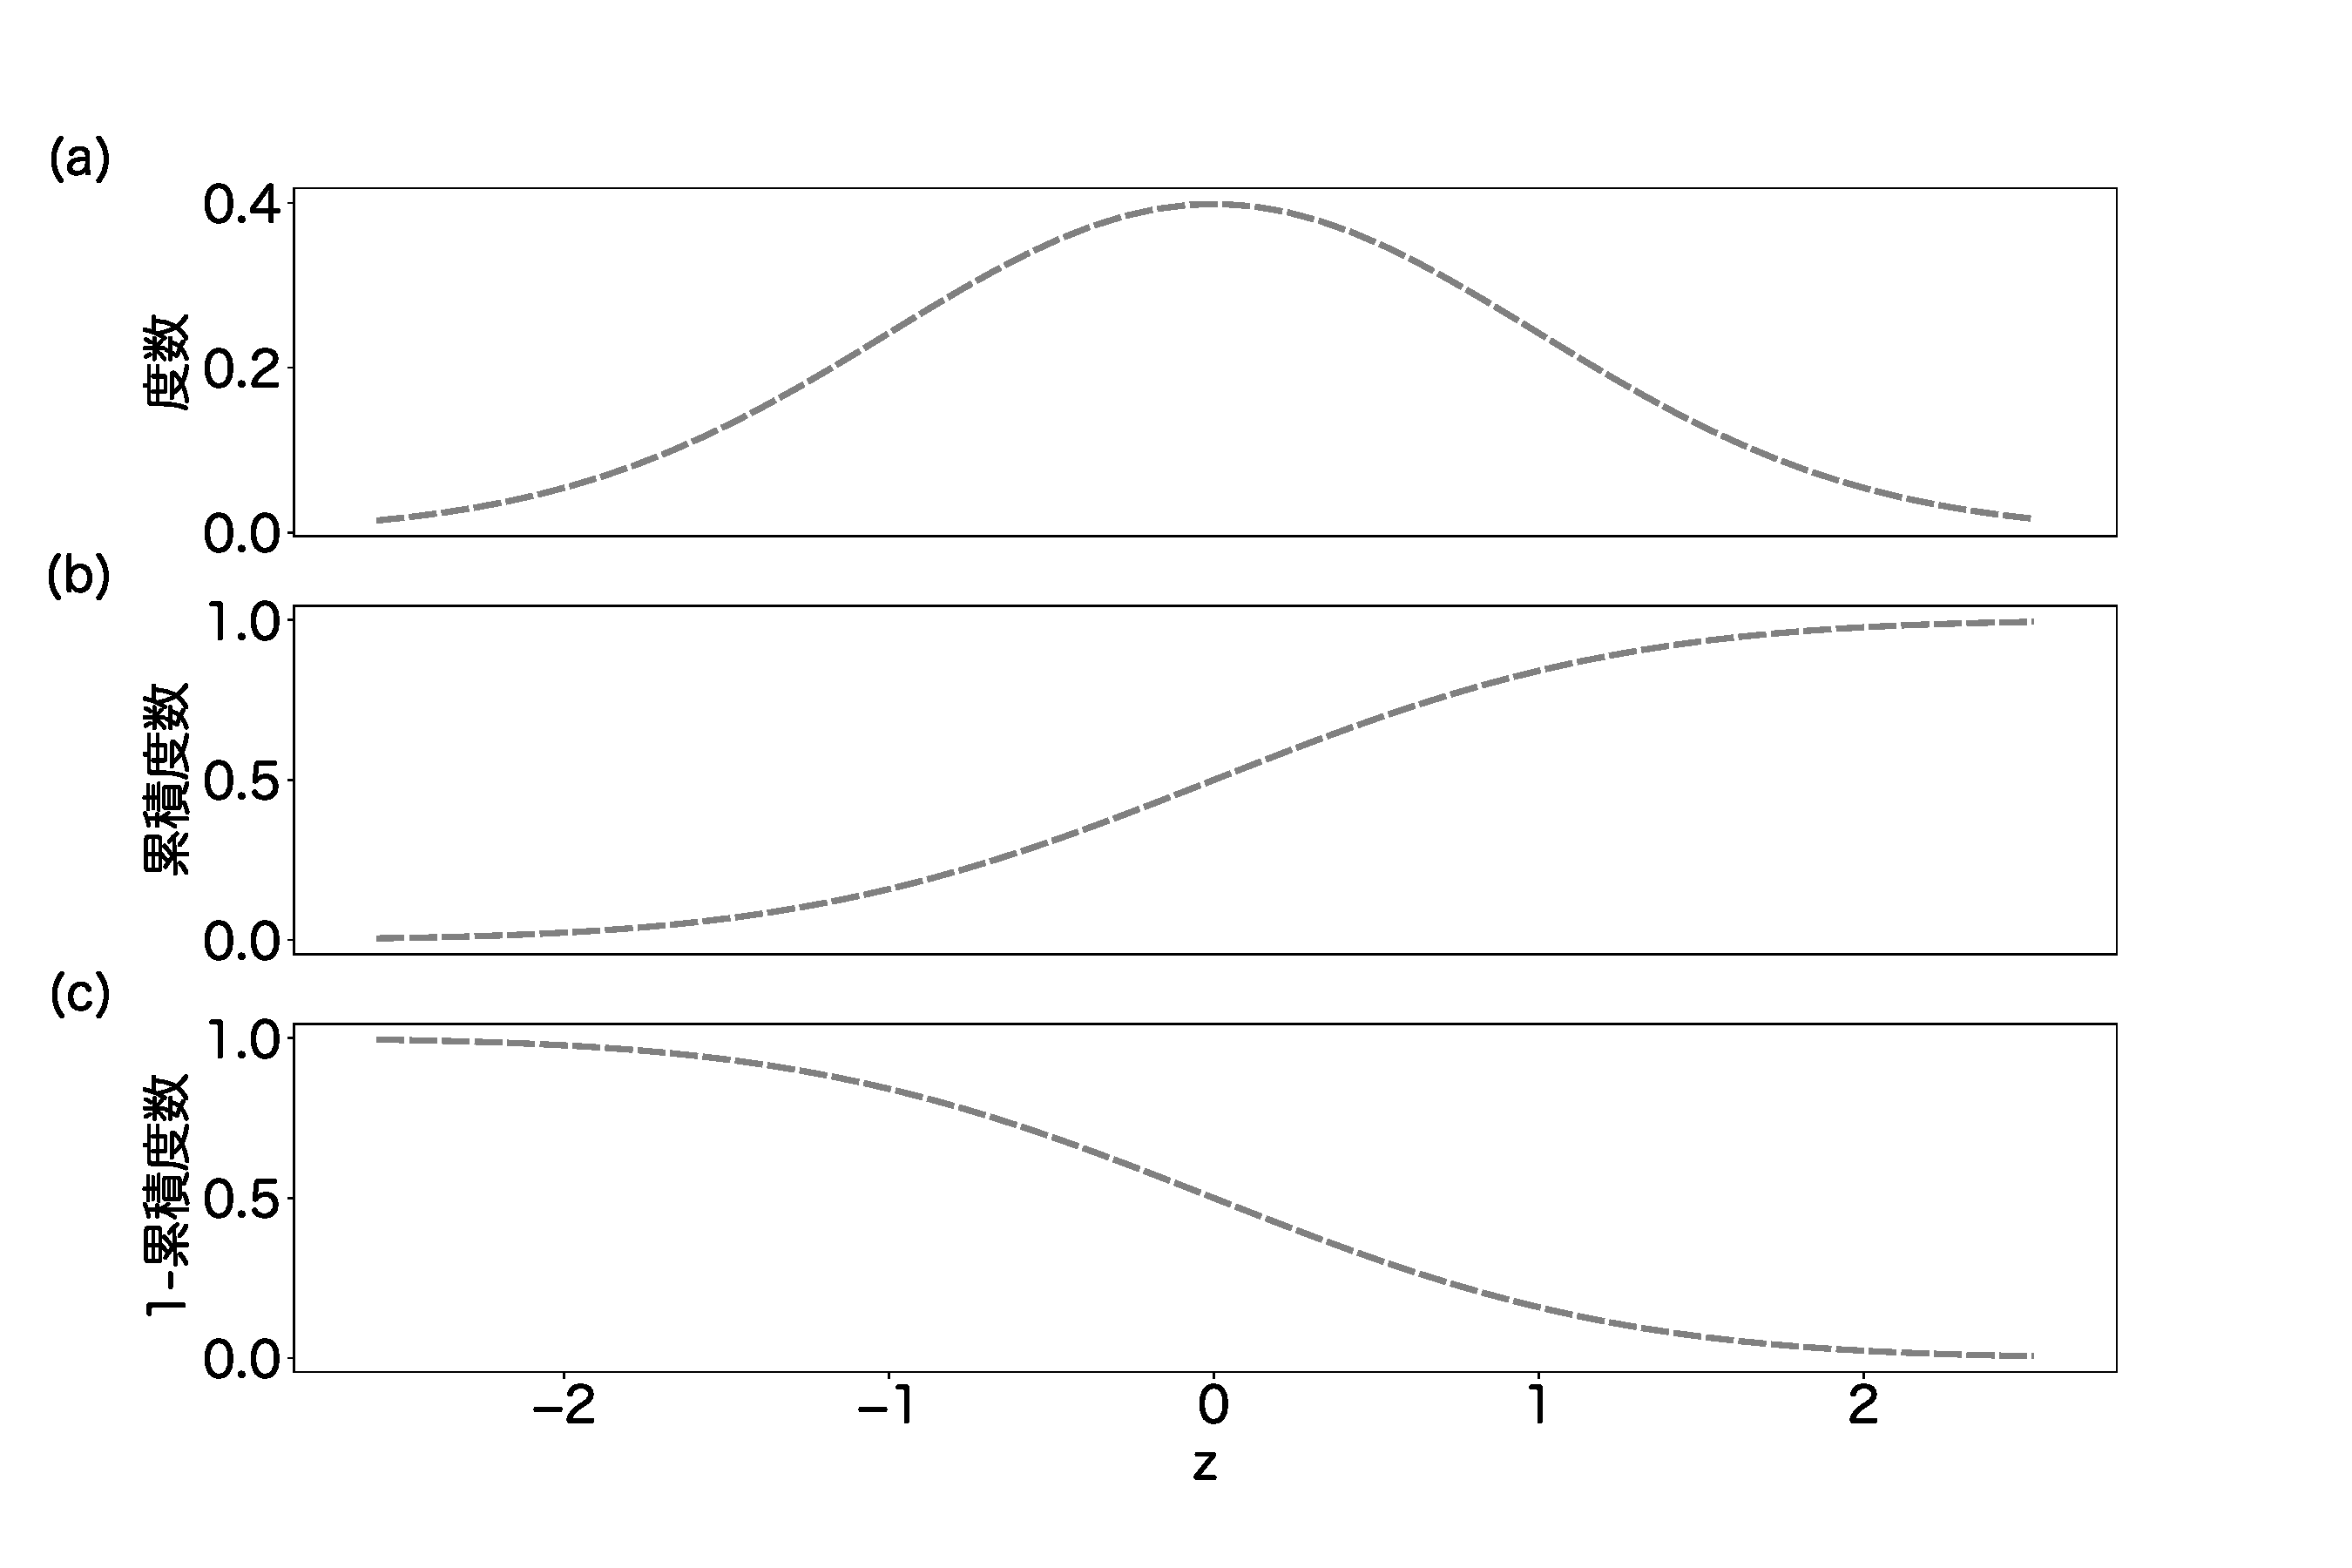
\includegraphics[width=15cm]{./image/02_/standard_normal.pdf}
        \caption{標準正規分布(a)確率密度関数(b)累積度数分布(c)1-累積度数分布}
        \label{fig:standard_normal_distribution}

    \end{center}
\end{figure}
    

\subsection{正規分布に従う確率変数の出現しやすさ1}
標準正規関数に従う確率変数が$95\%$の確率で見つかる範囲を求めてみます。
標準正規関数は、0を中心にして、対称な関数なので、正負の値が同じ程度の確率で見つかります。言い換えれば、$0\sim a$までの積分値と、$-a\sim 0$までの積分値が同じになります。そこで、次の積分を考えて、その最小値となる値を見つけてみます。
\begin{equation}
\int_{-a}^{a} \frac{1}{\sqrt{2\pi}}\exp(-\frac{z^2}{2}) dz = 0.95
\end{equation}

\begin{lstlisting}
b,a = norm.interval(0.95,0,1) # 積分値が0.95になる範囲を計算
print(norm.cdf(b, loc=0, scale=1)-norm.cdf(a, loc=0, scale=1)) # 0.95になるかを確認
print(b,a) # その範囲を表示
\end{lstlisting}


$0<\alpha<1$に対して、$\Phi(z_\alpha) = 1-\alpha$となる$z_\alpha$を上側$100\%$点という。
$z_{0.05}=1.64,z_{0.025}=1.96$の値は後でよく使う。

より、一般的には、$\alpha(0\leq \alpha \leq 0)$を指定すると、その半分$\alpha/2$となる積分範囲の末端を$a_1$とします。数式で書くと、
\begin{equation}
    \int_{-\infty}^{a_1} \frac{1}{\sqrt{2\pi}}\exp(-\frac{x^2}{2})dx = \frac{\alpha}{2}.
\end{equation}
同様に、右側の範囲の末端を$a_2$とします。数式で書くと、
\begin{equation*}
    \int_{a_2}^{\infty} \frac{1}{\sqrt{2\pi}}\exp(-\frac{x^2}{2})dx = \frac{\alpha}{2}.
\end{equation*}
これを書き換えると、次と同値です。
\begin{equation*}
    \int_{-\infty}^{a_2} \frac{1}{\sqrt{2\pi}}\exp(-\frac{x^2}{2})dx = 1-\frac{\alpha}{2}.
\end{equation*}

\begin{figure}
\begin{center}
    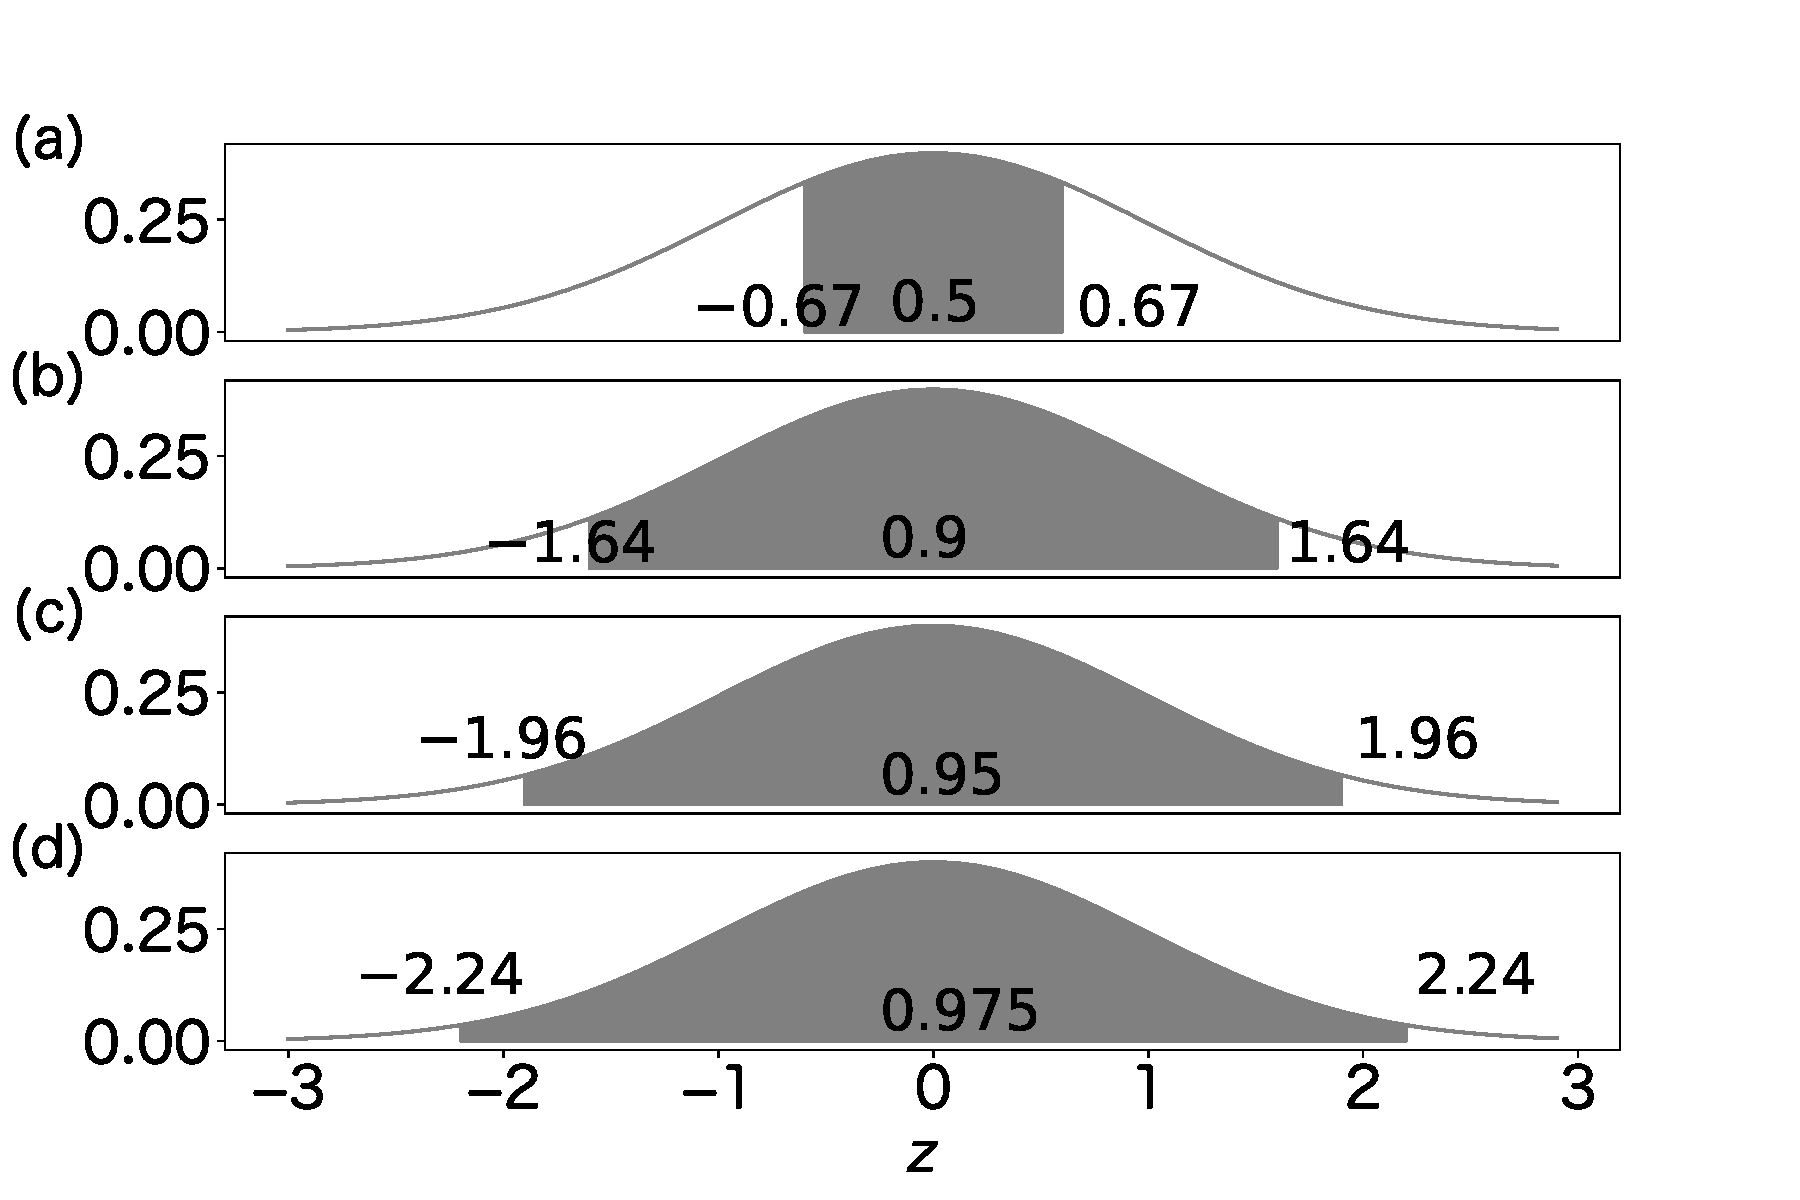
\includegraphics[width=15cm]{./image/02_/z_value.pdf}
    %\caption{図1.p値cm}
  \end{center}
\end{figure}

標準正規分布$z\sim N(0,1)$において$95\%$の確率で確率変数が見つかる範囲を調べることはできましたが、正規分布$x\sim N(\mu,\sigma^2)$においてでは、どの範囲になるのでしょう。次の定理を使えば簡単に計算ができます。
\begin{theo}
    確率変数$x$が、$x\sim N(\mu,\sigma^2)$であるならば、$\frac{x-\mu}{\sigma}\sim N(0,1)$である。    
\end{theo}
\begin{theo}
$\alpha(0\leq \alpha\leq 1)$に対して、$\int_{-\infty}^{z}\frac{1}{\sqrt{2\pi}}\exp(-x^2/2)=\alpha$を満たすとき、$\int_{-\infty}^{\mu+\sigma z} \frac{1}{\sqrt{2\sigma^2}}\exp(-\frac{(x-\mu)^2}{2\sigma})=\alpha$である。同様に、$\int_{z}^{-\infty}\frac{1}{\sqrt{2\pi}}\exp(-x^2/2)=1-\alpha$を満たす$z$について、$\int_{\mu+\sigma z}^{\infty} \frac{1}{\sqrt{2\sigma^2}}\exp(-\frac{(x-\mu)^2}{2\sigma})=1-\alpha$である。
\end{theo}
言い換えれば、標準正規分布の軸上の点$z$を、$[-\infty,z]$の範囲での積分値を保ったまま、正規分布$N(\mu,\sigma^2)$上の点に変換するには、$\frac{x-\mu}{\sigma}=z$を$x$について解けば良いことになります。

この定理により、以下をとけば、値が$95\%$の確率で得られる範囲がわかります。
\begin{eqnarray*}
    \frac{x-\mu}{\sigma}=z_{0.025}\\
    \rightarrow x = \mu+\sigma z_{0.025}
\end{eqnarray*}
また、
\begin{eqnarray*}
    \frac{x-\mu}{\sigma}=-z_{0.025}\\
    \rightarrow x = \mu-\sigma z_{0.025}
\end{eqnarray*}
以上により、$x \sim N(\mu,\sigma^2)$が$95\%$の確率で見つかる範囲は、$[\mu-\sigma z_{0.025},\mu+\sigma z_{0.025}]$であることがわかります。
同様に$90\%$の確率で見つかる範囲は、$[\mu-\sigma z_{0.05},\mu+\sigma z_{0.05}]$です。

\subsection{より大きな値をとる確率}
$x$を標準正規分布の確率変数とし、($x\sim N(0,1)$)また、$x\leq 0$であるとします。。$x$以上の大きな値を取る確率は、$P(X>x)=1-\varPhi(x)$で計算できます。
同様に、$x < 0$であるときは、より小さな値を取る値が、$P(x<X)=\varPhi(x)$で同様に計算できます。
図\ref{fig:z_value_larger}には、$x$に対して、より異なった値を取る確率を書いています。

$x$の大きさ$|x|$よりも大きな値を取る確率は、以上の二つの和で次のようにかけます。
\begin{equation}
    P(|x|>z) = 1-\varPhi(|x|)+\varPhi(-|x|)
\end{equation}
式を見ると正の数で$x$より大きな値を取る確率と、負の数で$x$より小さな値を取る確率の和になっていることが確認できます。
$P(|x|>z)$はより極端な値を取る確率などと言う方もされます。

計算してみます。$x=1.64$であれば、$\varPhi(1.64)=0.95$より、それ以上に大きな値を得る確率は、$P(X>1.64)=0.05$です。また、$x=-1.64$であれば、$\varPhi(-1.64)=0.05$です。よって、$|x|=|1.64|$よりも大きな値を得る確率は$P(|1.64|>X)=0.1$です。


\begin{figure}
    \begin{center}
        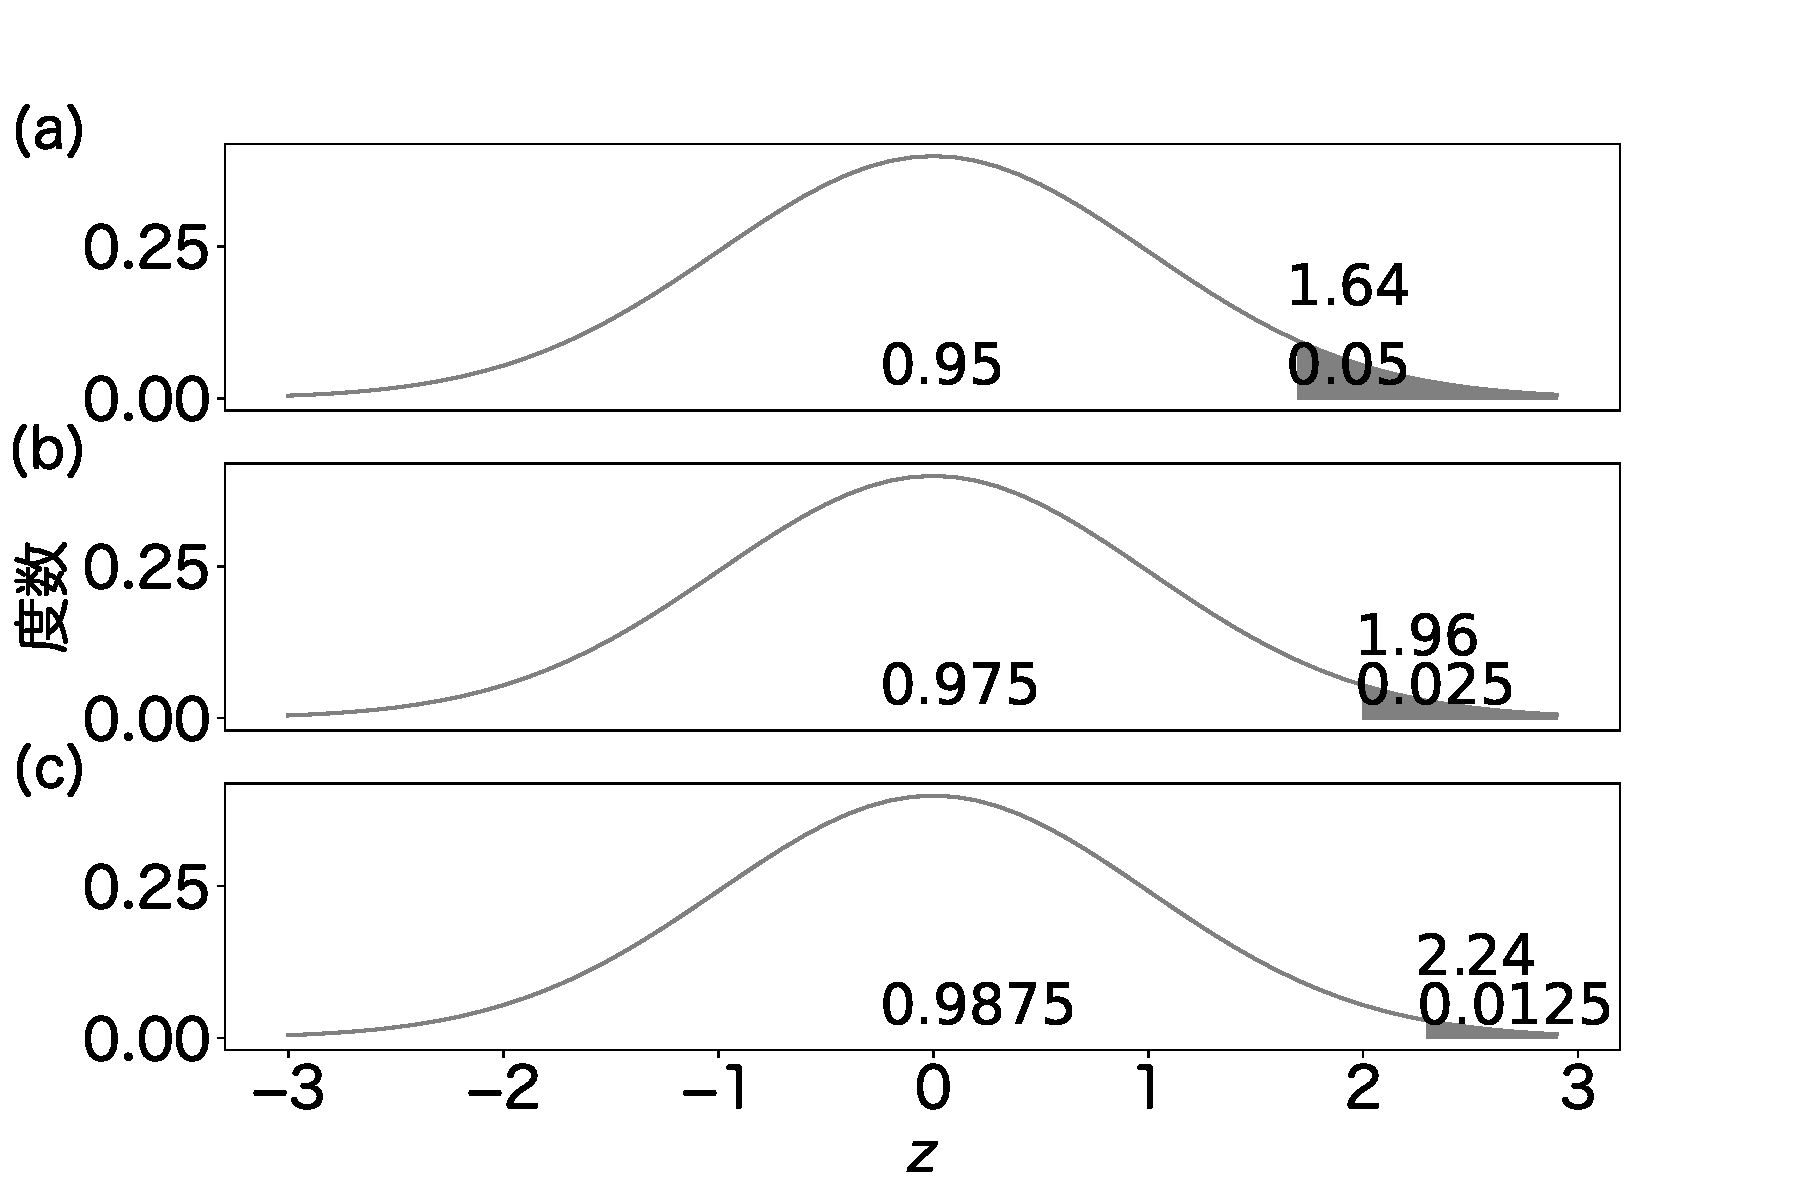
\includegraphics[width=15cm]{./image/02_/z_value_larger.pdf}
        \caption{標準正規分布におけるより大きな値(より偏った値)を取る確率。(a)$z=1.64$より大きな値を取る確率は0.05。(b)$z=1.96$より大きな値を取る確率は$0.025$。(c)$z=2.24$よりも大きな値を取る確率は$0.0125$}
        \label{fig:z_value_larger}
      \end{center}
    \end{figure}

\subsection{$N(0,1)$での珍しい値は、$N(0,2)$では珍しくない?}
以上の議論により、$N(0,1)$において、$z=1.64$以上の値が出る確率はおよそ$5\%$である。
では、$N(0,2)$において$z=1.64$が出る確率はいくつだろうか。
$N(0,2)$において、$z=1.64\times2$以上に大きな値が出る確率は、およそ$5\%$である。
このことから、$N(0,2)$において$z=1.64$以上の値が出る確率は、$5\%$より大きいことがわかる。
具体的に、計算をしてみると、その確率は$0.206$程度であることがわかる。
\begin{lstlisting}
1-norm.cdf(1.64,0,2)
\end{lstlisting}

\subsection{$N(1.96,1)$で出てくる値は、$N(0,1)$において珍しい?}
$N(1.96,1)$において、$1.96$以上の値が出る確率は、$50\%$です。明らかに、よく出る値であることがわかります。
一方で、$N(0,1)$においては、$1.96$以上の値が出る確率は、$2.5\%$くらいなので、珍しい値になります。
このように、確率分布の母数が変化すると、珍しい値も変化します。




\subsection{正規分布に従う確率変数の出現しやすさ2}
確率変数のしやすさを表す基準として、$\sigma$を基準にして、定数$a$倍の範囲$[\mu-a\sigma,\mu+a\sigma]$を使う方法もあります。
標準正規分布では、分散が$1$なので、その$0.5$倍、$1$倍、$2$倍、$3$倍の範囲はそれぞれ$[-0.5,0.5]$,$[-1,1]$,$[-2,2]$,$[-3,3]$になります。この範囲に入る確率は、それぞれ$0.38$,$0.683$,$0.954$,$0.997$です。それぞれの範囲と確率は、図\ref{fig:sigma_interval_probability}に図示しました。

$\sigma$の定数倍の範囲に値が見つかる確率は、$\sigma$の大きさに依存しないことが証明できます。言い換えれば、$[-0.5\sigma,0.5\sigma],[-\sigma,\sigma],[-2\sigma,2\sigma],[-3\sigma,3\sigma]$の範囲に値がある確率は、上記と同じで、それぞれおよそ$0.38$,$0.683$,$0.954$,$0.997$になります。


\begin{figure}
    \begin{center}
        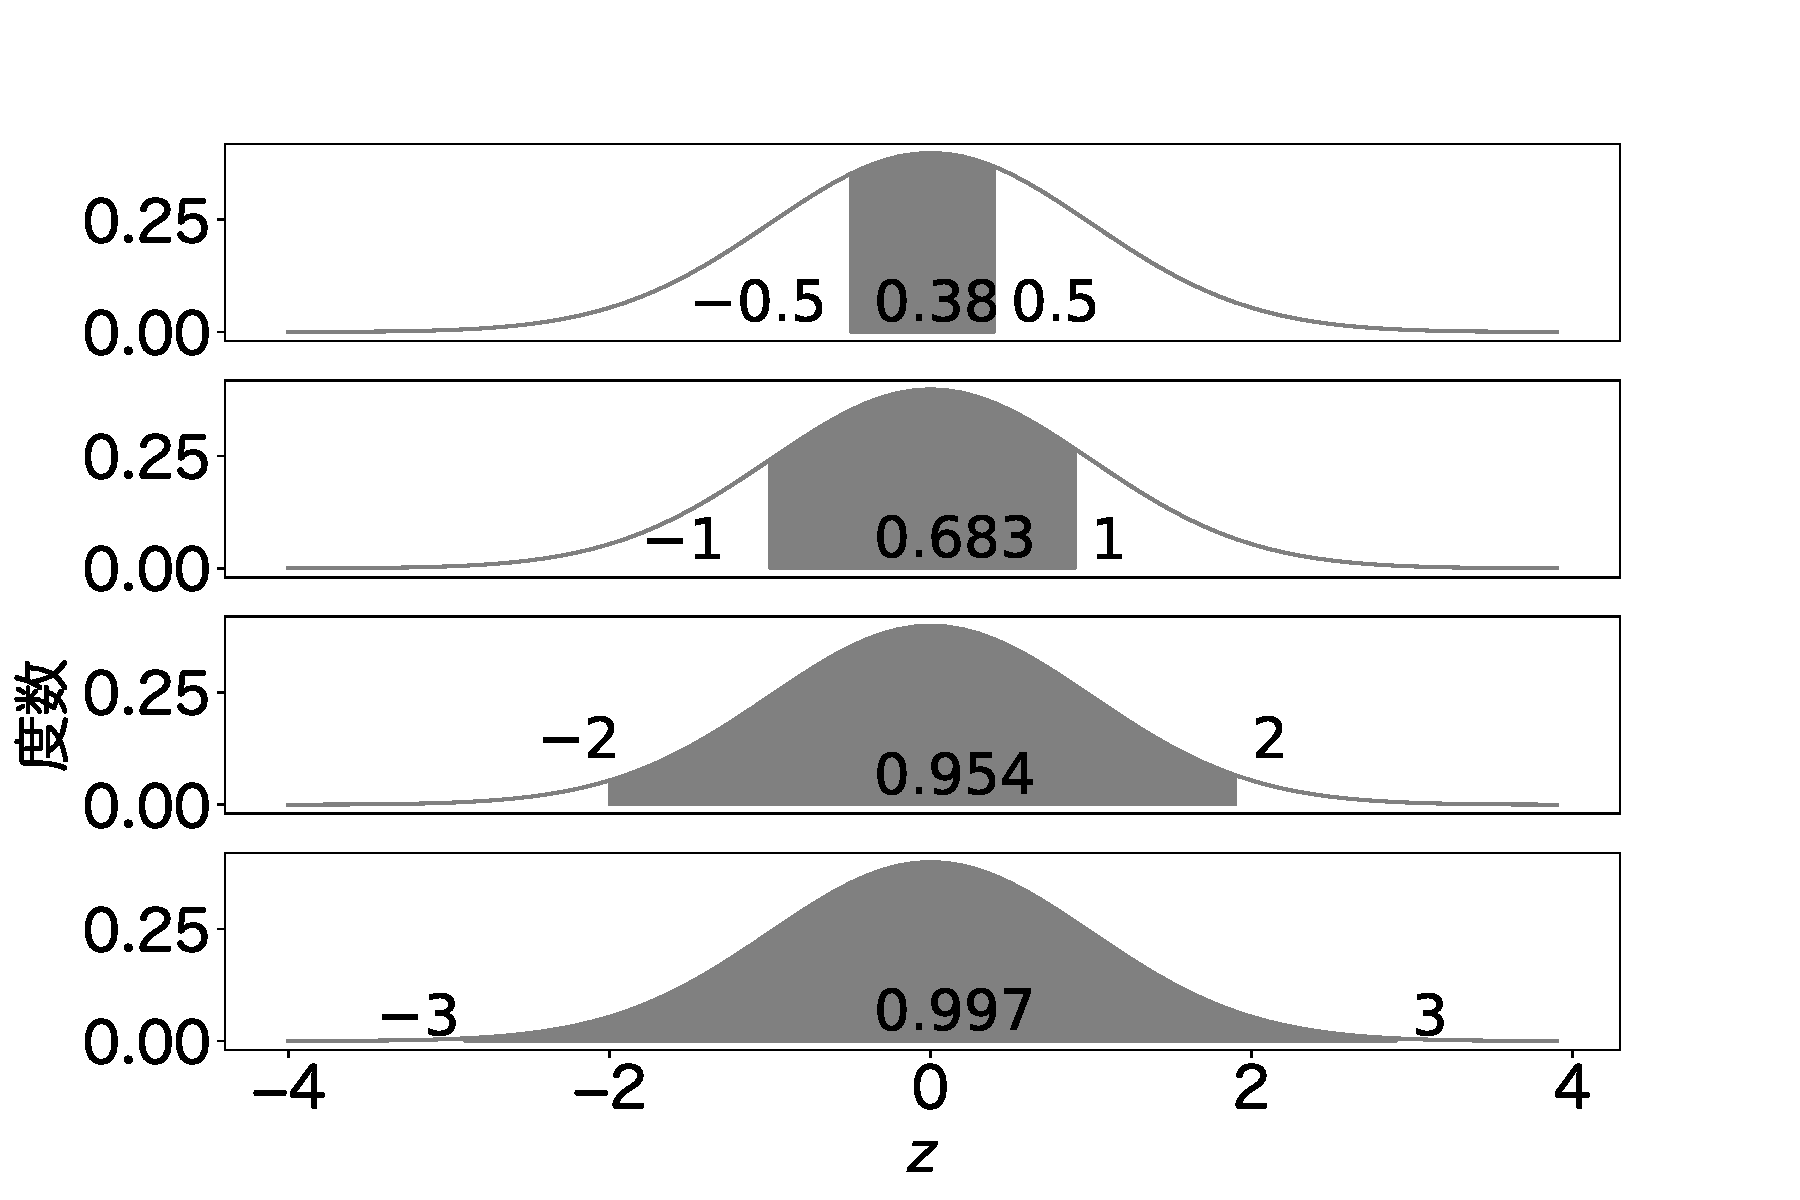
\includegraphics[width=15cm]{./image/02_/sigma_value.pdf}
        %\caption{図1.p値cm}
        \label{fig:sigma_interval_probability}
      \end{center}
\end{figure}

\begin{table}[hbtp]
    \caption{$\sigma$を基準にした値の出やすさ}
    %\label{table:data_type}
    \centering
    \begin{tabular}{lcr}
        \hline
        出現確率  & $N(0,1)$  &  $N(\mu,\sigma^2)$ \\
        \hline \hline
        0.38 & [-0.5,0.5]  & $[\mu-0.5\sigma,\mu+0.5\sigma]$ \\
        0.683 & [-1,1] & $[\mu-\sigma,\mu+\sigma]$\\
        0.954 & [-2,2] & $[\mu-2\sigma,\mu+2\sigma]$\\
        0.996 & [-3,3] & $[\mu-3\sigma,\mu+3\sigma]$\\
    \end{tabular}
\end{table}




\section{指数分布}
確率変数$X$が指数分布に従うことを$X \sim Exp(\lambda)$と書く。
指数分布の確率密度関数は、
\begin{equation*}
    f(x)=\lambda \exp(-\lambda x).
\end{equation*}
ここで、$\lambda$は、$\lambda>0$であり、指数分布の母数である。
期待値は$E[X]=\frac{1}{\lambda}$で、分散は、$V[X]=\frac{1}{\lambda^2}$である。
累積分布関数は、
\begin{equation*}
    F(x)=1-\exp(-\lambda x).
\end{equation*}
正規分布は、母数平均を中心として、左右対称に分布していた。言い換えれば、$\phi(\mu+x)=\phi(\mu-x)$である。一方で、指数分布は、左右非対称に分布が広がり、小さな値は大きな値よりも出現確率が高いので、$f(E[X]+a)\neq f(E[X]-a)$である。
また、正規分布では、母数平均と母数分散がそれぞれ独立なので、それぞれの特徴を独立に動かすことで、期待値や分散が独立に変化する。
指数分布では、母数が一つであり、母数を変化させると、期待値と分散は同時に変化する。



\begin{figure}
    \begin{center}
        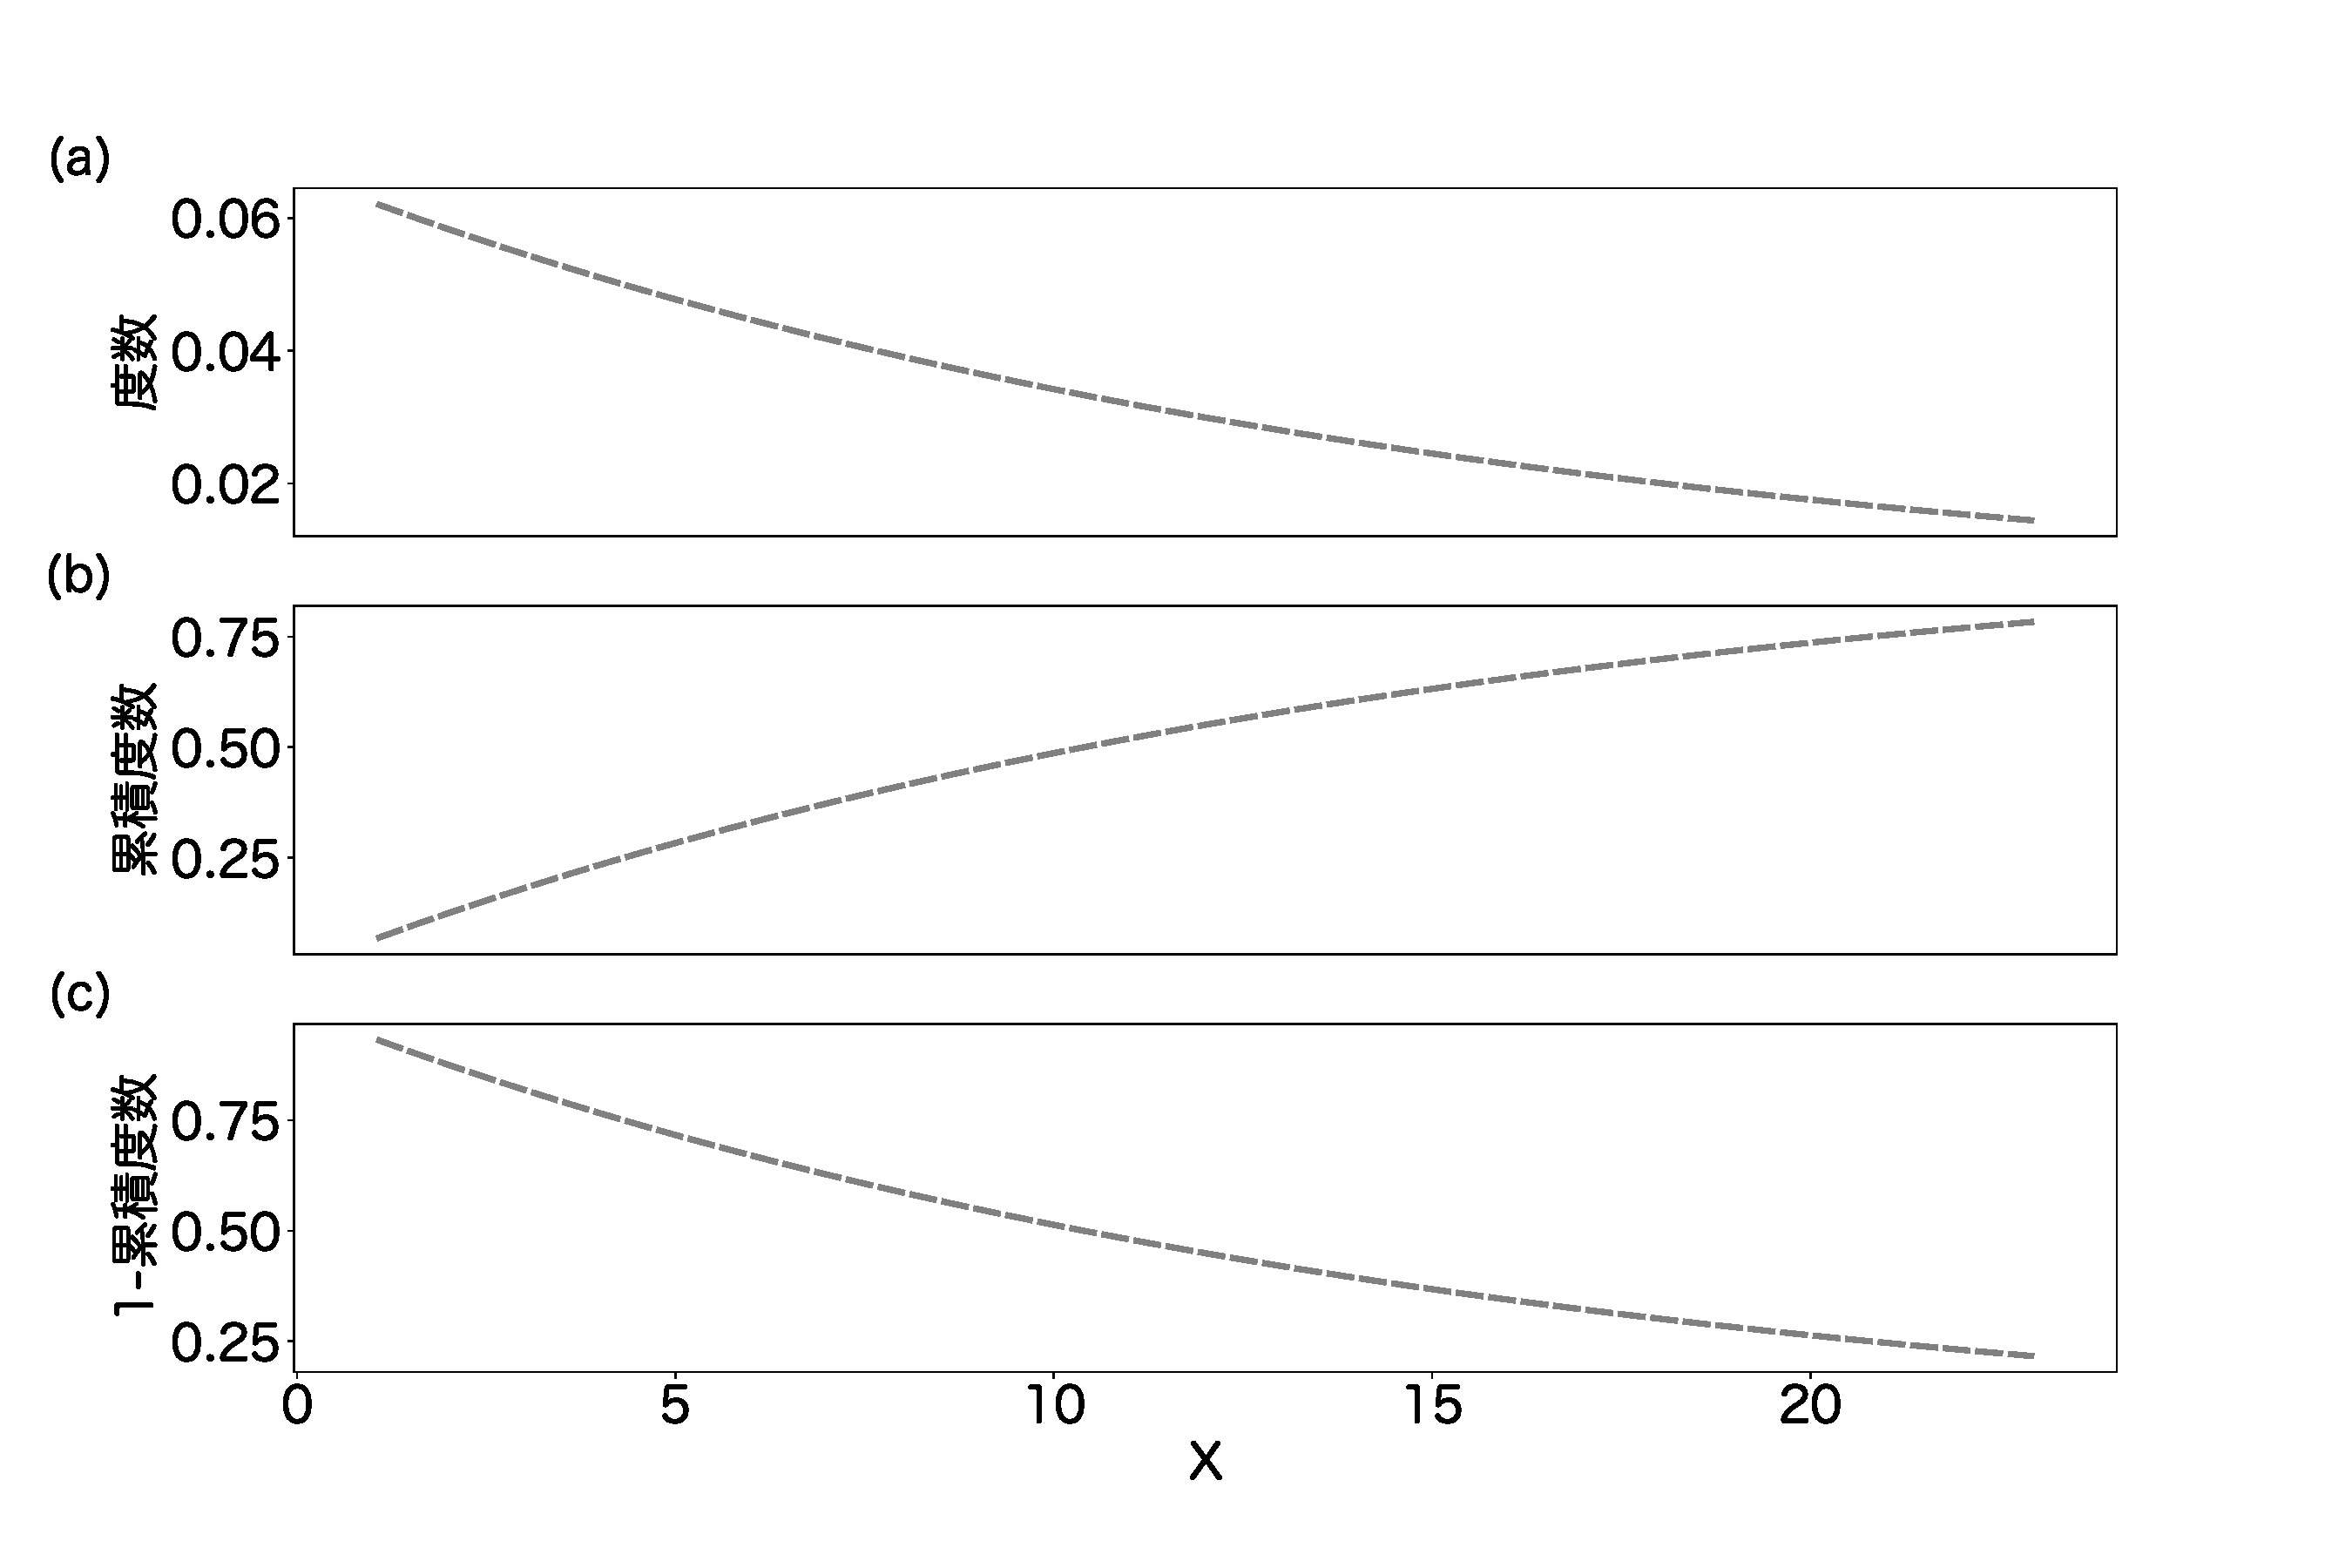
\includegraphics[width=15cm]{./image/02_/expon_frequency.pdf}
        \caption{指数分布$\lambda=1/15$(a)確率密度関数(b)累積度数分布(c)相補累積度数分布}
        \label{expon_frequency}
    \end{center}
\end{figure}


\subsection{指数分布に従う確率変数の出現しやすさ}
指数分布の確率密度関数を区間$[a,b]$で積分したときに、$\alpha(0\leq \alpha \leq 1)$になる$[a,b]$を求めます。条件として、
\begin{eqnarray*}
    \int_0^{a}  \lambda\exp(-\lambda x )dx &=& \alpha/2\\
    \int_0^{b} \lambda\exp(-\lambda x )dx &=& 1-\alpha/2
\end{eqnarray*}
を満たすとする。
$a$について、とくと、
\begin{eqnarray*}
    \int_0^{a}  \lambda\exp(-\lambda x )dx &=& \alpha/2\\
     1-\exp(-\lambda a) &=& \frac{\alpha}{2}\\
     \rightarrow a&=& \frac{1}{\lambda} \log\frac{1}{1-\alpha/2}
\end{eqnarray*}
$b$については、同様に、
\begin{equation*}
    b = \frac{1}{\lambda}\log\frac{\alpha}{2}
\end{equation*}
以上より、この積分の条件で、$100(1-\alpha)\%$の確率で値を得る範囲は、$[\frac{1}{\lambda} \log\frac{1}{1-\alpha/2} ,\frac{1}{\lambda}\log\frac{\alpha}{2}]$である。
図\ref{fig:expon_simulation_sample}は、指数分布により、サンプルサイズ$1000$の標本を$100$回作って、各標本においてデータが区間$[\frac{1}{\lambda} \log\frac{1}{1-\alpha/2} ,\frac{1}{\lambda}\log\frac{\alpha}{2}]$に入った割合をシミュレーションし、そのヒストグラムを表示している。確かに、$95\%$くらいの割合でその区間にデータが入っている。


\begin{figure}
    \begin{center}
        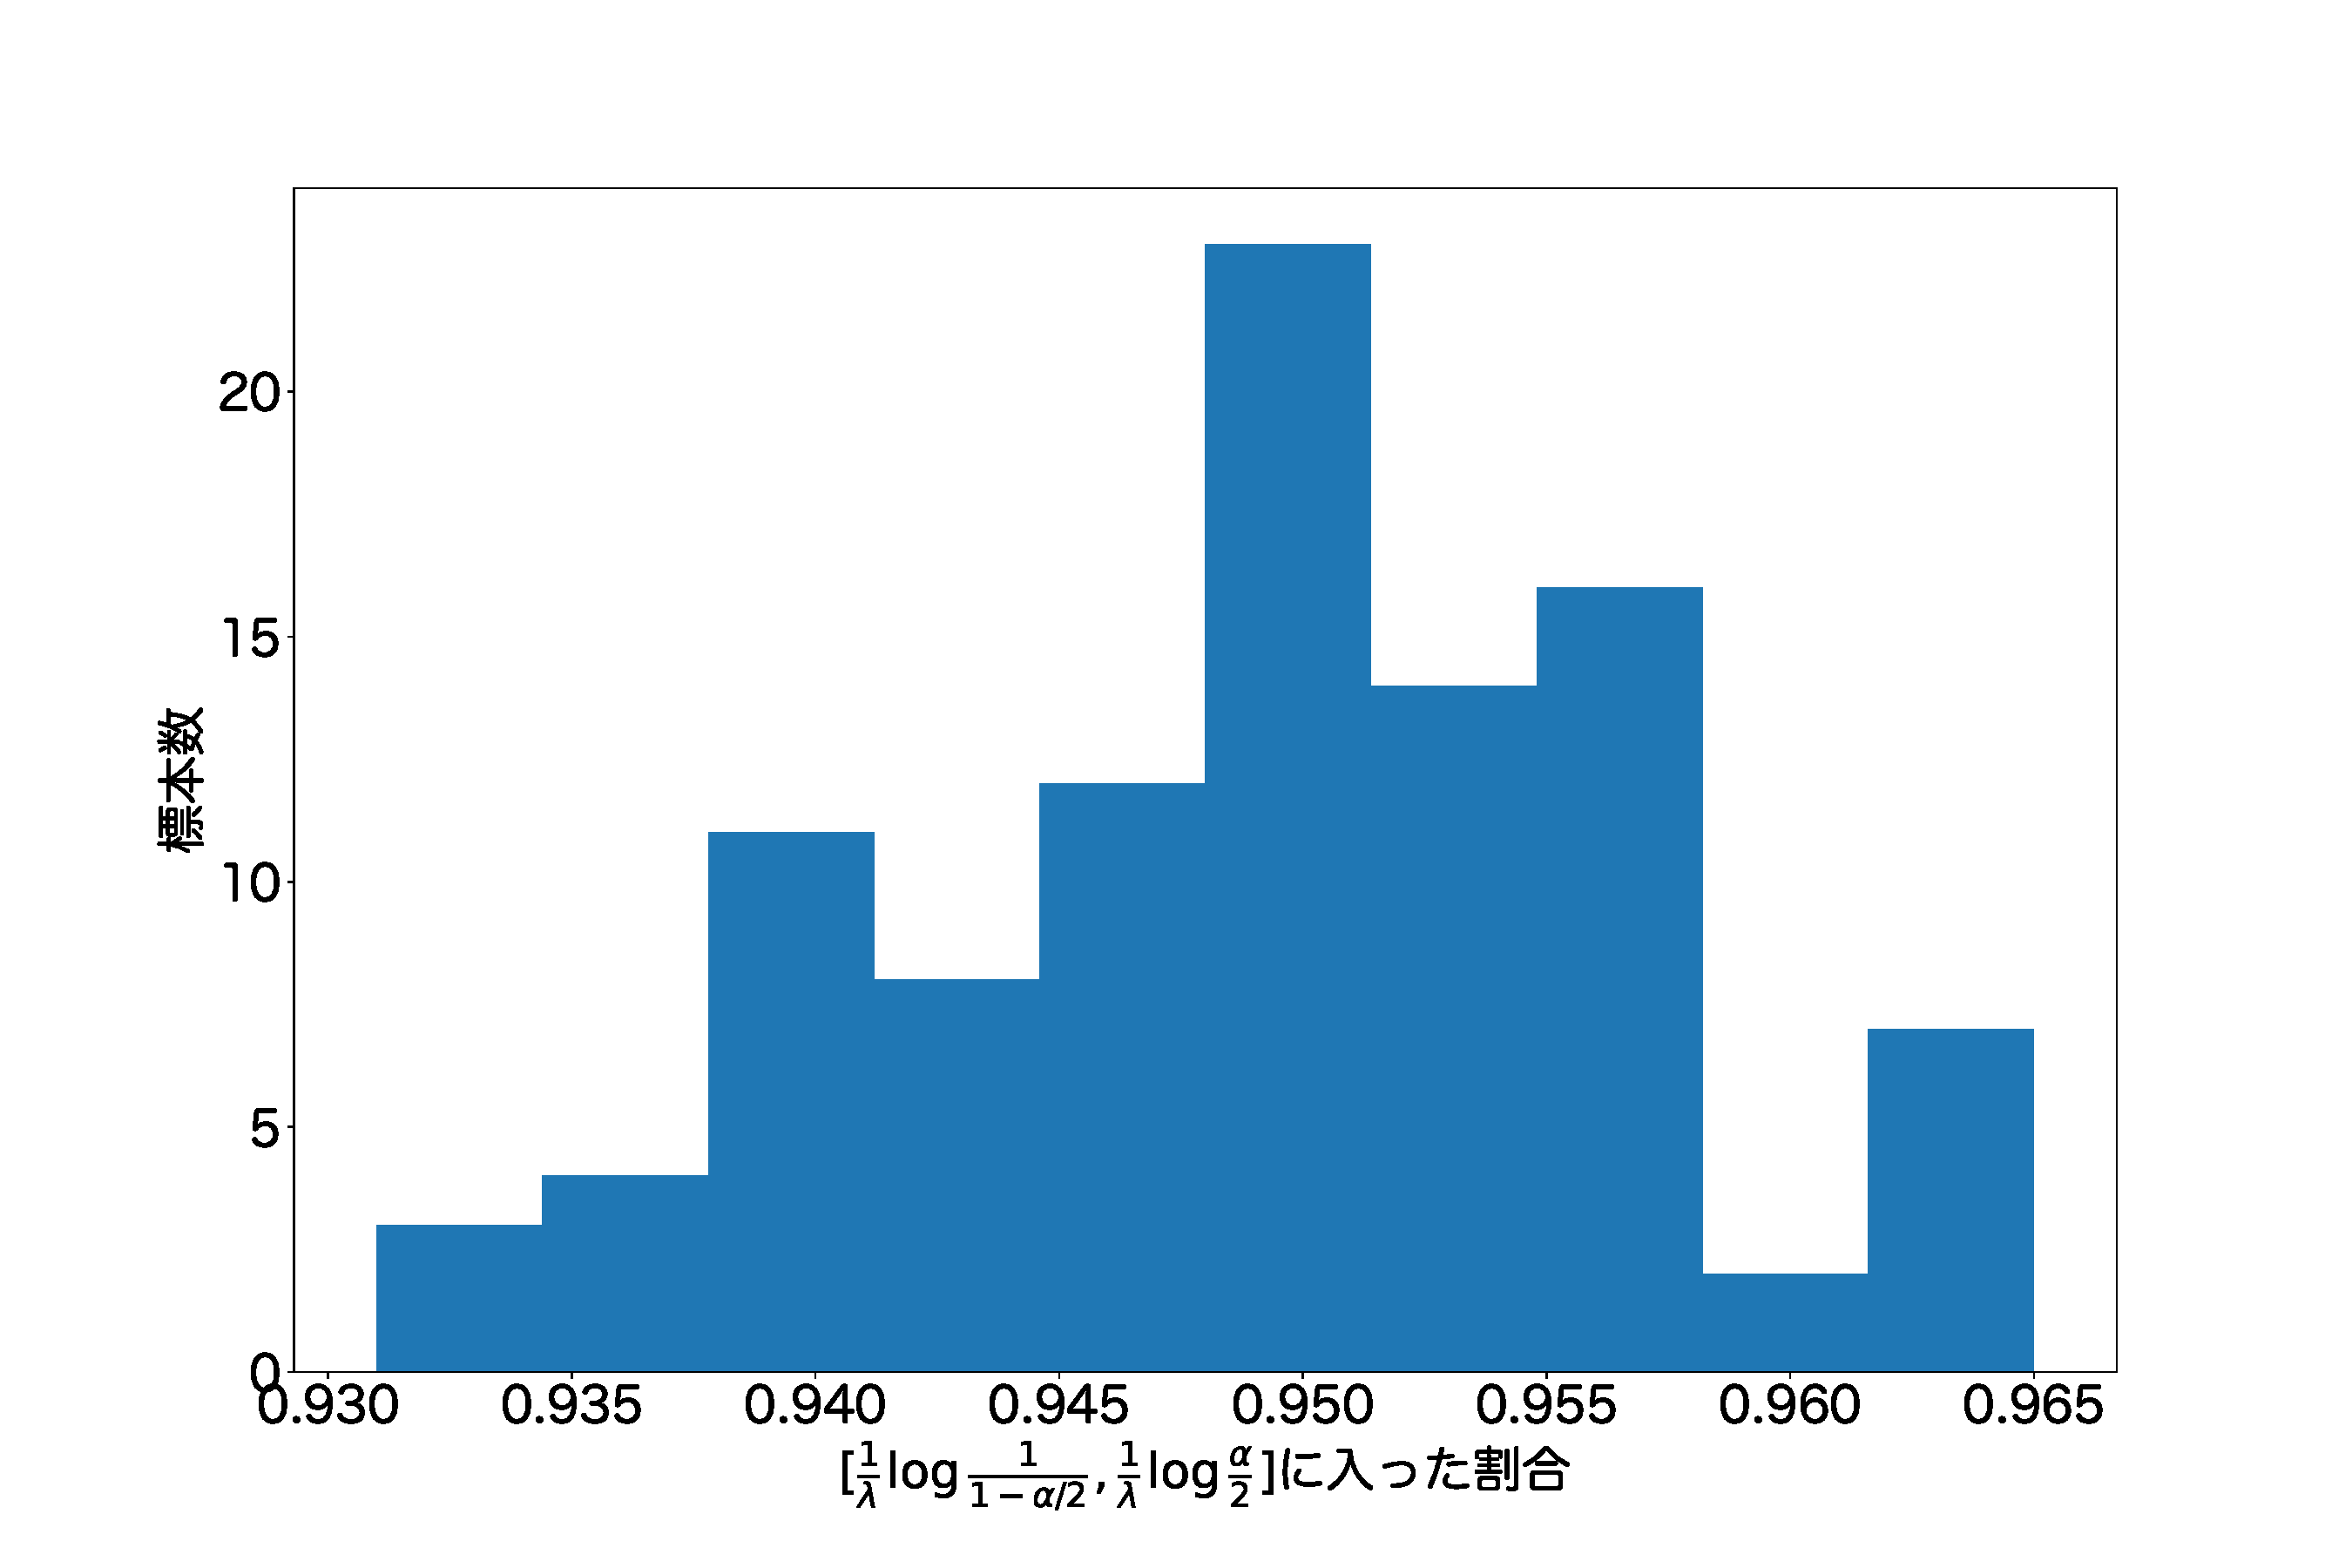
\includegraphics[width=15cm]{./image/02_/expon_simulation_sample.pdf}
        \caption{指数分布$\lambda=1/10$からサンプルサイズ1000の標本を100回シミュレーションし、各標本においてデータが区間$[\frac{1}{\lambda} \log\frac{1}{1-\alpha/2} ,\frac{1}{\lambda}\log\frac{\alpha}{2}]$に入った割合を計算した。そのヒストグラム。}
        \label{fig:expon_simulation_sample}

    \end{center}
\end{figure}


\section{カイ二乗分布}
確率変数$X$がカイ二乗分布に従うことを$X \sim \chi^2_k$と書く。ここで、$k$はカイ二乗分布の母数で、自由度を示し、自然数を取る。
確率密度関数は、
\begin{equation*}
    f(x;k) = \frac{1}{2^{k/2}\Gamma(k/2)}x^{k/2-1}\exp\left(-\frac{x}{2}\right).
\end{equation*}
ここで、$\Gamma(k/2)$はガンマ関数を表す\footnote{$ \Gamma(z)=\int_0^{\infty }t^{z-1}\exp(-t)dt$である。 }。
累積分布間数は、
\begin{equation*}
    F(x) = \frac{\gamma(k/2,x/2)}{\Gamma(k/2)}.
\end{equation*}
ここで、$\gamma(k/2,x/2)$は、不完全ガンマ関数である\footnote{$\gamma(a,x)=\int_0^x t^{a-1}\exp^{-t}dt$である。ガンマ関数も、不完全ガンマ関数も計算できなくても問題はない。コンピュータを使えばすぐに計算してくれる。}。
この関数も左右非対称である。


\begin{figure}
    \begin{center}
        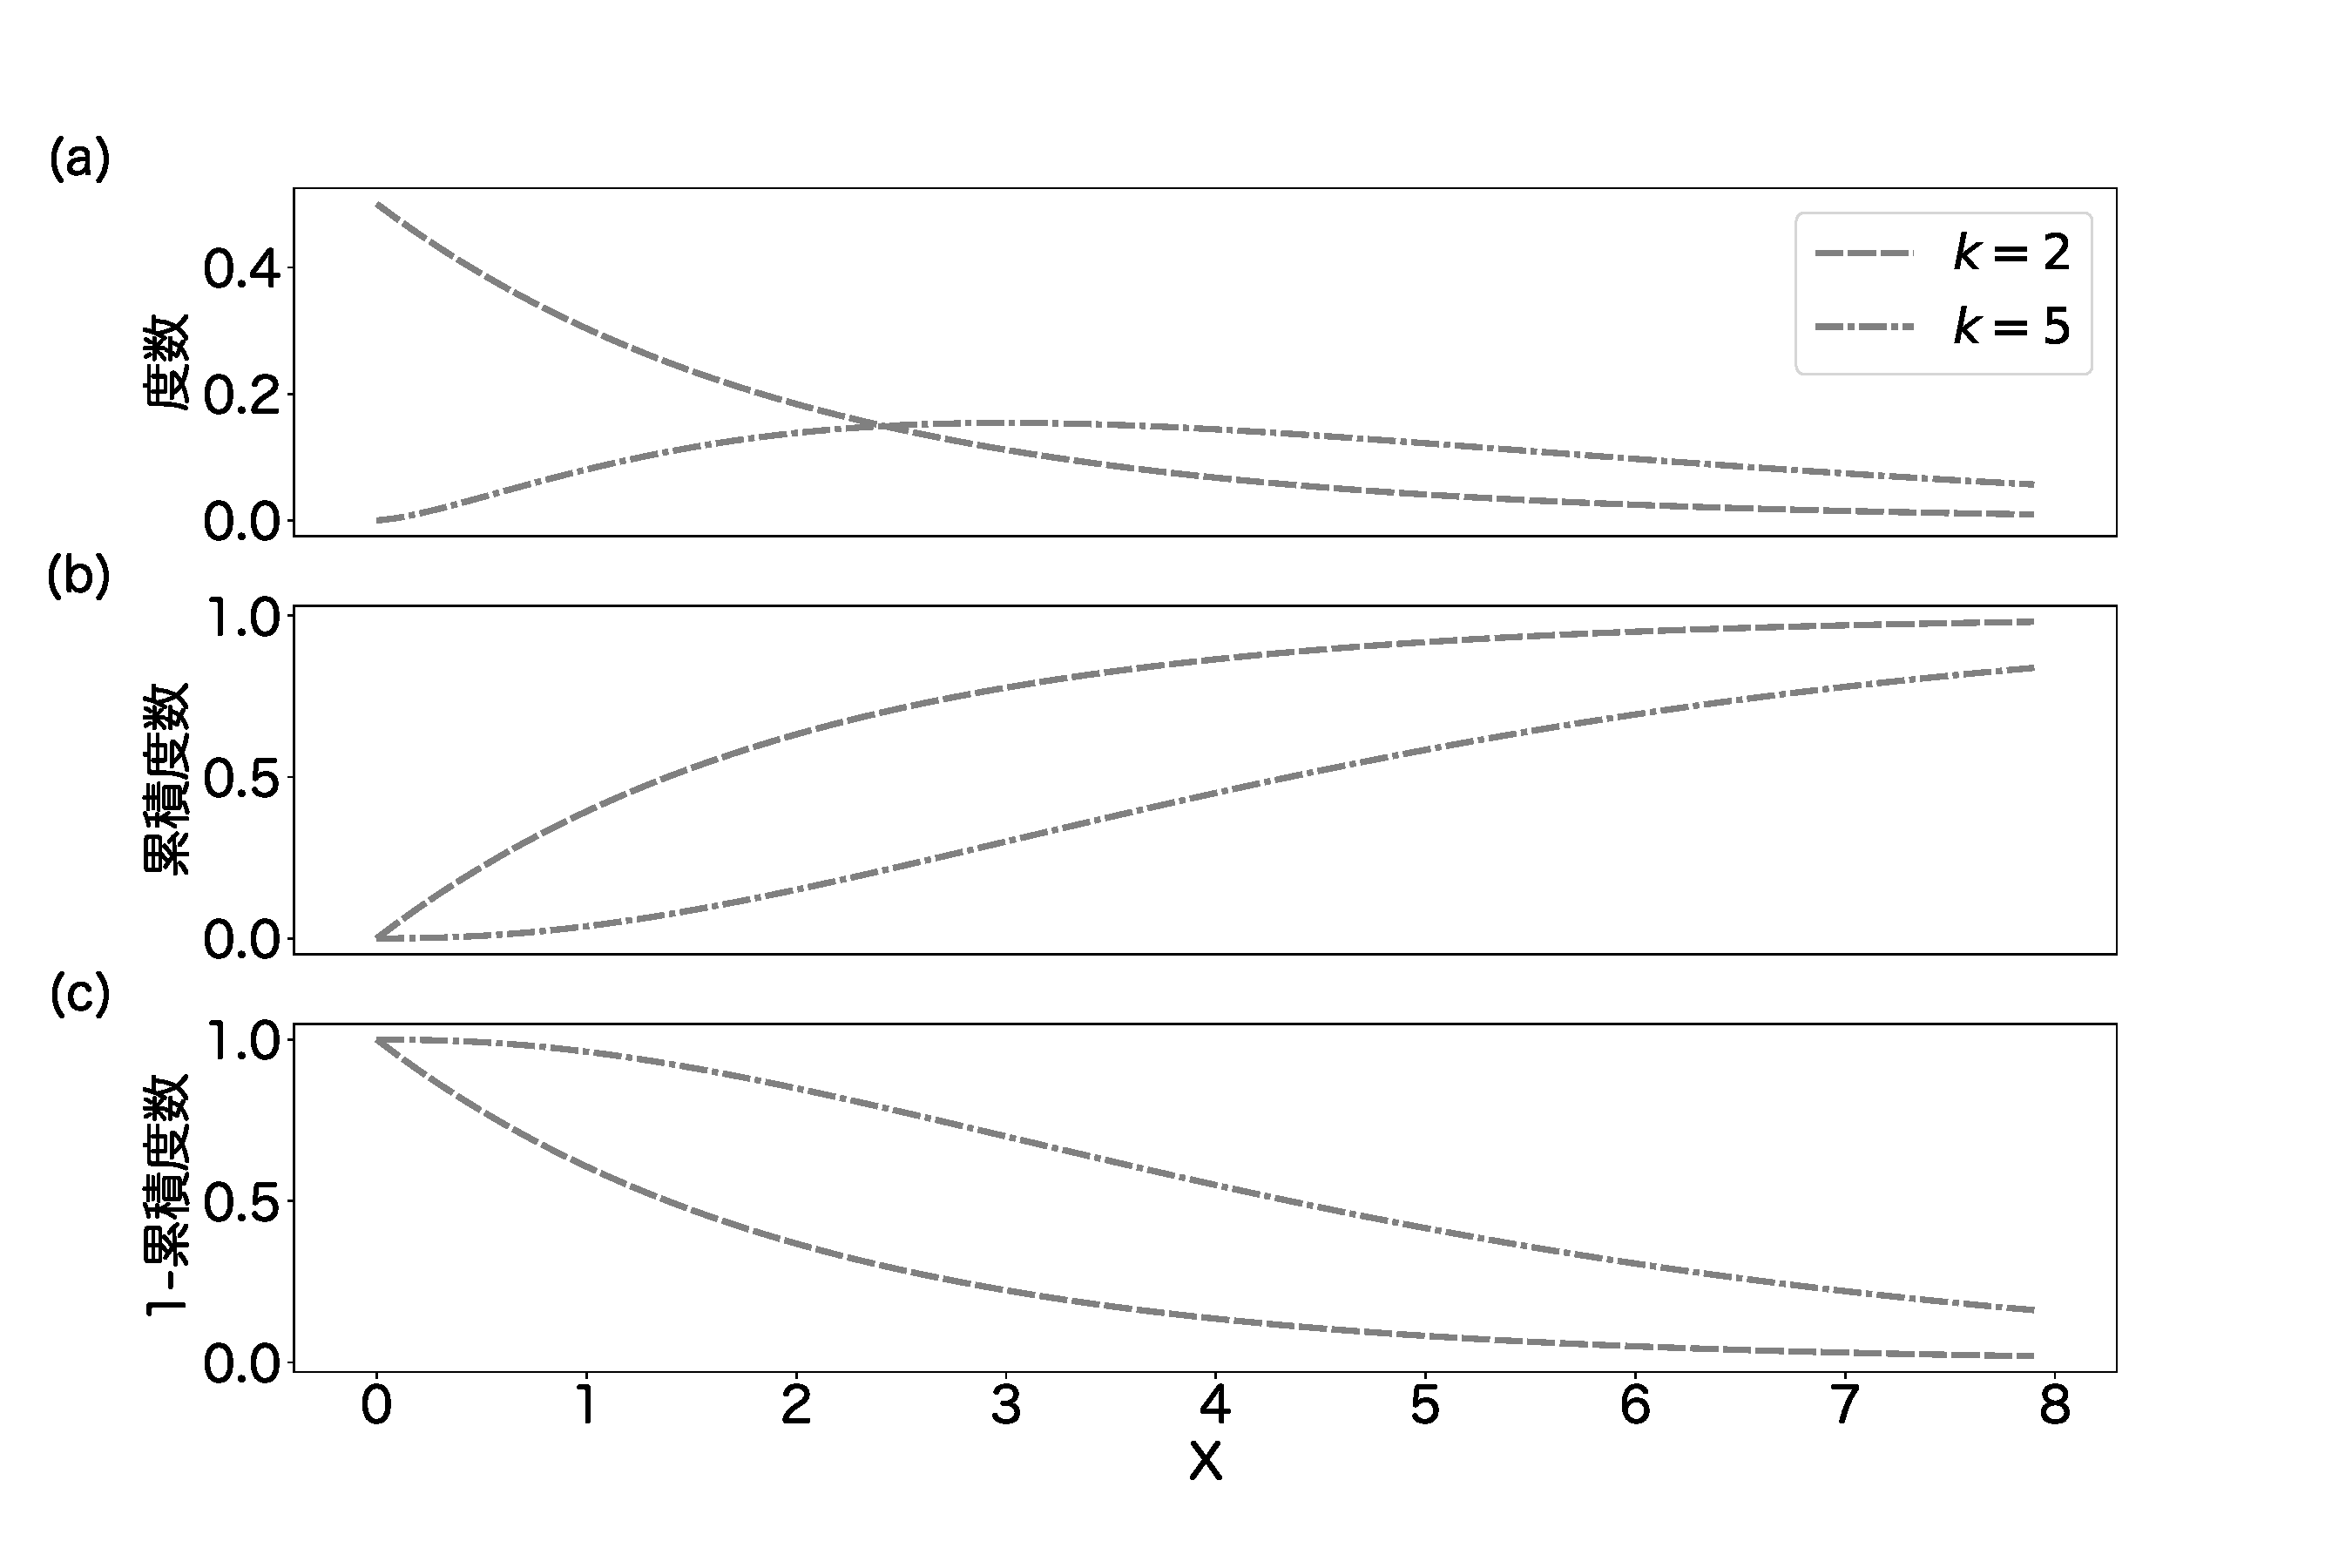
\includegraphics[width=15cm]{./image/02_/chi2_frequency.pdf}
        \caption{カイ二乗分布}
        \label{chi2_}
    \end{center}
\end{figure}

\subsection{カイ二乗分布に従う確率変数の出現しやすさ}
カイ二乗分布の確率密度関数を区間$[a,b]$で積分したときに、$\alpha(0\leq \alpha \leq 1)$になる$[a,b]$を求めます。条件として、
\begin{eqnarray*}
    \int_0^{a}  \frac{1}{2^{k/2}\Gamma(k/2)}x^{k/2-1}\exp\left(-\frac{x}{2}\right)dx &=& F(a)-F(0) = \alpha/2\\
    \int_0^{b} \frac{1}{2^{k/2}\Gamma(k/2)}x^{k/2-1}\exp\left(-\frac{x}{2}\right)dx &=& F(b)-F(0)= 1-\alpha/2
\end{eqnarray*}
を満たすとする。
代数的に$a,b$について解くことが難しいので、数値的に計算してみた結果を載せておく(表\ref{table:chi2_confidence})。この$a,b$をそれぞれ$\chi^2_k(\alpha),\chi^2_{k}(1-\alpha)$と書くことがある。


\begin{table}[hbtp]
    \caption{$\alpha=0.05$}
    \label{table:chi2_confidence}
    \centering
    \begin{tabular}{lcc}
    %\hline
    k  & $a$   & $b$   \\
    \hline \hline
    1 &  0.0009 &  5.02\\
    3 & 0.215 & 9.3484  \\
    5 &  0.831 & 12.832 \\
      \hline
    \end{tabular}
  \end{table}

\section{$t$分布}
確率変数$T$が$t$分布に従うとき、$T \sim t(\nu)$と表記する。
確率密度関数は、
\begin{equation*}
    f(t) = \frac{\Gamma((\nu+1)/2)}{\sqrt{\nu \pi}\Gamma(\nu/2) }(1+t^2/\nu)^{-(\nu+1)/2}.
\end{equation*}
ここで、$\nu$は、$0$より大きな実数である。
この関数を見ただけでは、すぐには判別するのは難しいかもしれないが、$f(t)$には$t$が関係する部分は$(1+t^2/\nu)$だけである。二乗の項があるので、偶数関数であることがわかり、$0$を中心にした対称な関数$f(t)=f(-t)$であることがわかる。
累積分布関数は著者には難しすぎるので、記述しない。wikipediaなどで調べれば正しそうな数式が書かれている。



\begin{figure}
    \begin{center}
        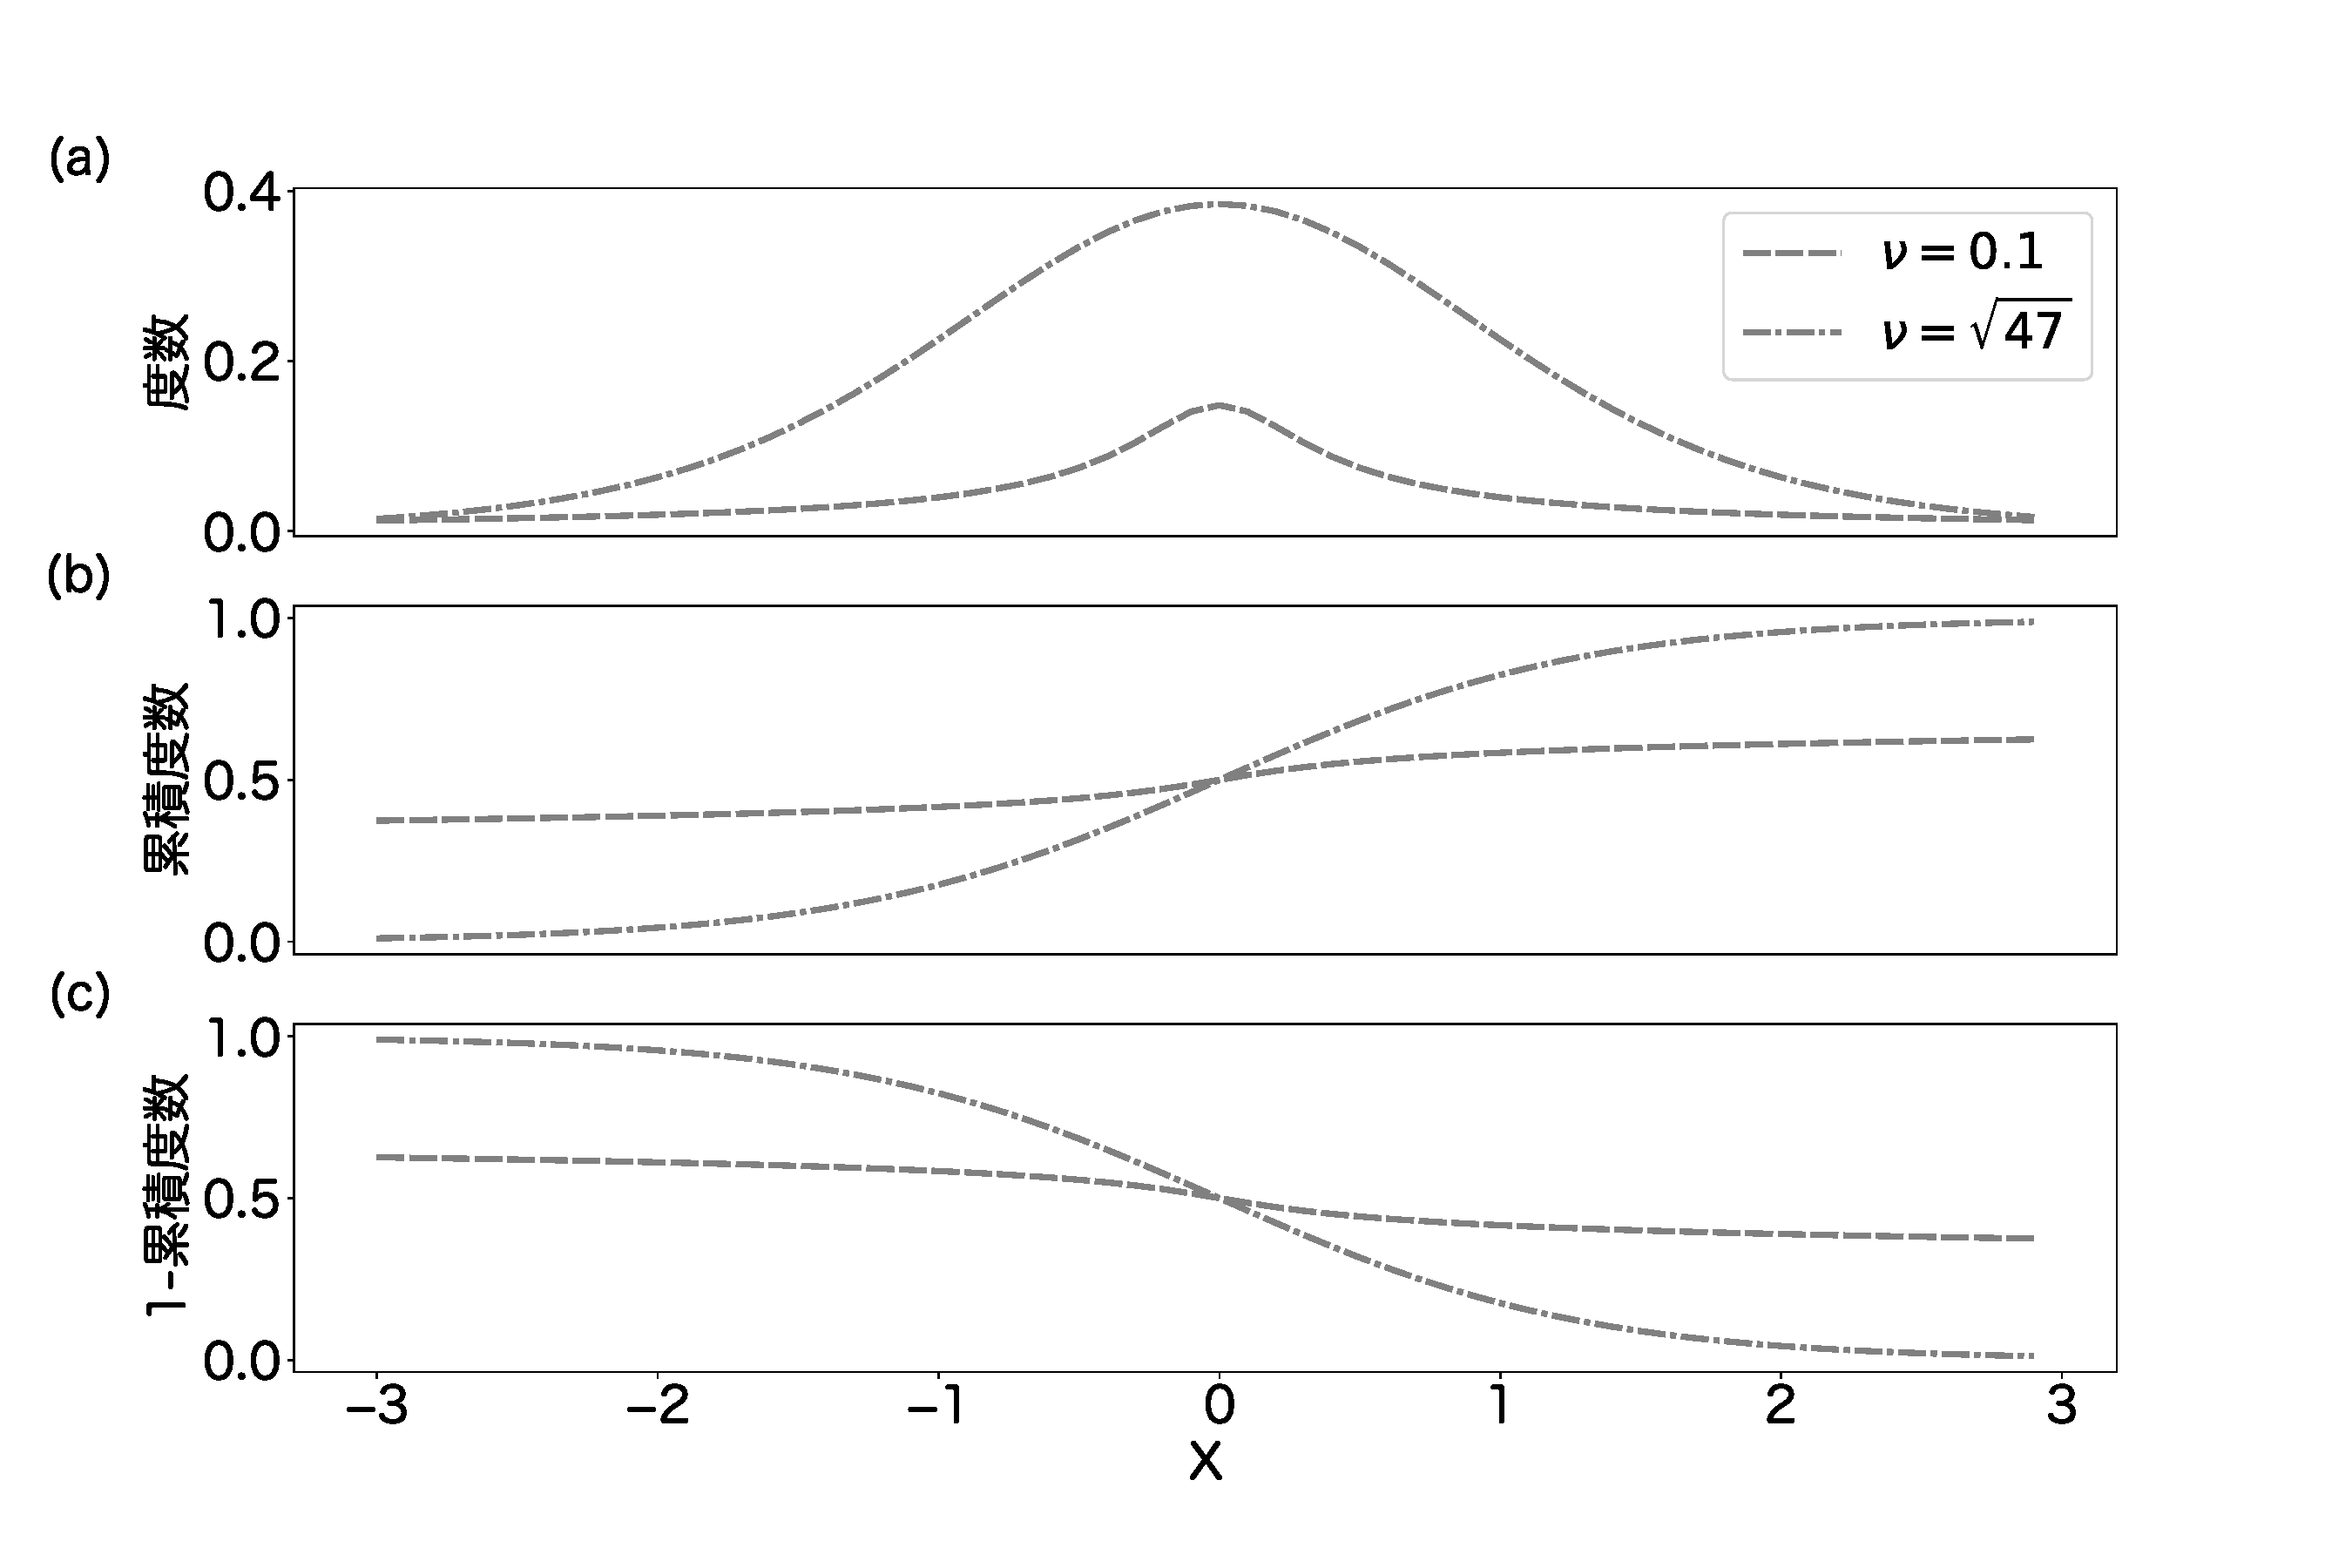
\includegraphics[width=15cm]{./image/02_/student_t_frequency.pdf}
        \caption{t分布}
        \label{student_t}
    \end{center}
\end{figure}

\subsection{$t$分布における珍しい値}
$t$分布における$|T|$以上の値が得られる確率が$\alpha$程度になる$|T|$のリスト。
例えば、$n=10$の$t$分布において$|T|=1.81$以上の値が得られる確率は、$0.1$程度である。


\begin{table}[hbtp]
    \caption{$t$分布における$|T|$以上の値が得られる確率が$\alpha$程度になる$|T|$のリスト}
    \label{table:student_t_confidence}
    \centering
    \begin{tabular}{cccc}
    %\hline
    n & p=0.1 & $p=0.05$ & $p=0.025$   \\
    \hline \hline
    1 & 6.31 & 12.70 & 25.45 \\
    5 & 2.01 &2.57  & 3.16\\
    10 & 1.81 &  2.22& 2.63 \\
      \hline
    \end{tabular}
  \end{table}
% https://bellcurve.jp/statistics/course/8968.html


\section{統計分布の関係}
同一の確率分布からサンプリングされた複数の確率変数$X_1,X_2,\cdots,X_n$を得たとき、それを要約した要約統計量がどのような分布関数に従うのかを考察する。
% $(\star)$のついた項目は、科学的(恣意的)な判断を含んでいる。

\subsection{正規分布の再生性}
$X \sim N(\mu_1,\sigma^2_1),Y\sim(\mu_2,\sigma^2_1)$とするとき、$aX+bY \sim N(a\mu_1+b\mu_2,a^2\sigma^2_1+b^2\sigma^2_2)$より、$a=\frac{1}{2},b=\frac{1}{2}$。すると、$\frac{X}{2}+\frac{Y}{2}\sim N(\frac{\mu_1+\mu_2}{2},\frac{\sigma^2_1}{2^2}+\frac{\sigma^2_2}{2^2})$である。$\mu_1=\mu_2,\sigma_1=\sigma_2$とすると、$\frac{X+Y}{2}\sim N(\mu_1,\frac{\sigma^2_1}{2})$が成り立つ。
このことを利用すると、$X_1,X_2,\cdots,X_n\sim N(\mu,\sigma^2)$とすると、$\bar{X}=\frac{X_1+X_2+\cdots+X_n}{n}\sim N(\mu,\frac{\sigma^2}{n})$である。よって$\frac{\bar{X}-\mu}{\sqrt{\frac{\sigma^2}{n}}}\sim N(0,1) $。また、$\bar{x}$の出現しやすい区間は、
\begin{equation*}
    -z_{0.025}<\frac{\bar{X}-\mu}{\sqrt{\frac{\sigma^2}{n}}} < z_{0.025}
\end{equation*}
である。式を変形すると、
\begin{equation*}
    \mu-z_{0.025}\frac{\sigma^2}{n}<\bar{x}<\mu+z_{0.025}\frac{\sigma^2}{n}
\end{equation*}
がわかる。
以上をまとめておく。

\begin{theo}
    $X_1,X_2,\cdots,X_n \sim N(\mu,\sigma^2)$とすると、$\frac{\bar{X}-\mu}{\sqrt{\frac{\sigma^2}{n}}}\sim N(0,1)$ ただし、$\bar{X}=\frac{X_1+X_2+\cdots+X_n}{n}$。また、$\bar{X}$の出現しやすい区間は、$\mu-z_{0.025}\frac{\sigma^2}{n}<\bar{x}<\mu+z_{0.025}\frac{\sigma^2}{n}$である。
\end{theo}



\begin{theo}
    $X_1,X_2,\cdots,X_{n_1} \sim N(\mu_1,\sigma_1^2),Y_1,Y_2,\cdots,Y_{n_2}\sim N(\mu_2,\sigma_2^2)$ただし、$\mu_1\neq \mu_2,\sigma_1\neq \sigma_2$とする。正規分布の再生性により、$\bar{X}\sim N(\mu_1,\frac{\sigma^2_1}{n_1}),\bar{Y}\sim N(\mu_2,\frac{\sigma^2_2}{n_2})$である。次が成り立つ。
    $\bar{X}-\bar{Y} \sim N(\mu_1-\mu_2,\frac{\sigma^2_1}{n_1}+\frac{\sigma^2_2}{n_2})$であり、
    \begin{equation*}
        \frac{(\bar{X}-\bar{Y})-(\mu_1-\mu_2)}{\sqrt{\frac{\sigma_1^2}{n_1}+ \frac{\sigma_2^2}{n_2}}}\sim N(0,1).
    \end{equation*}
\end{theo}



\subsection{指数分布の再生性}
指数分布$Exp(\lambda)$と、ガンマ分布$Ga(1,\frac{1}{\lambda})$は、同一の密度分布関数であり、それは$f(x) = \frac{1}{\lambda} \exp(-\frac{x}{\lambda})$である。ガンマ分布には、分布の再生性があり、$X\sim Ga(a_1,b),Y\sim Ga(a_2,b)$であるなら、$X+Y \sim Ga(a_1+a_2,b)$である。このことを、$n$個の確率変数$X_1,X_2,\cdots X_n \sim Exp(\lambda)(=Ga(1,\frac{1}{\lambda}) )$に適用すると、$X_1+X_2+\cdots+X_n \sim Ga(n,\frac{1}{\lambda})$である。以上によって、$n\bar{X}\sim Ga(n,\frac{1}{\lambda})$ただし、$\bar{X}=X_1+X_2+\cdots+X_n$である。
再生性については、確率母関数を利用することで証明できる。

\begin{theo}
    $X_1,X_2,\cdots,X_n \sim Ga(1,\frac{1}{\lambda})$ならば、
    $n\bar{X}\sim Ga(n,\frac{1}{\lambda})$
\end{theo}

\begin{proof}
    $Ga(1,\frac{1}{\lambda})$の確率母関数は、$M_X(t)=(1-\frac{1}{\lambda}t)^{-1}$である。確率変数$X_1+X_2+\cdots+X_n$の確率母関数は
    \begin{eqnarray}
        M_{n\bar{X}} = M_{X_1+X_2+\cdots+X_n} &=& M_{X_1}M_{X_2}\cdots M_{X_n} \\
        &=& (1-\frac{1}{\lambda}t)^{-1}(1-\frac{1}{\lambda}t)^{-1}\cdots(1-\frac{1}{\lambda}t)^{-1}\\
        &=& (1-\frac{1}{\lambda}t)^{-n}
    \end{eqnarray}
    以上より、$n\bar{x}\sim Ga(n,\frac{1}{\lambda})$である。
\end{proof}

\if 0
\subsubsection{対数正規分布の再生性}
$X\sim \Lambda(\mu_1,\sigma_1^2), Y\sim \Lambda(\mu_2,\sigma^2_2)$とするとき、$XY\sim\Lambda(\mu_1+\mu_2,\sigma_1^2+\sigma_2^2)$である。
これを使えば、$X_1,X_2,\cdots,X_n \sim \Lambda(\mu,\sigma^2)$について、その積$X_1,X_2\cdots X_n \sim \Lambda(n\mu,n\sigma^2)$である。

ここで、$X_1X_2\cdots X_n$は十分統計量にならないので、検定が作れないのか?
一方で、$\log X_1+\log X_2 \cdots \log X_n $は十分統計量$N(\mu,\sigma^2)$に従う。
$\log X_1^2+\log X_2^2 \cdots \log X_n $は十分統計量$\chi^2$分布に従う
% https://stats.stackexchange.com/questions/202890/jointly-sufficient-statistic-question
% https://mcm-www.jwu.ac.jp/~konno/pdf/statr28.pdf
% https://www.stats.ox.ac.uk/~reinert/stattheory/solutions109.pdf
% https://pages.stern.nyu.edu/~wgreene/MathStat/old-exam-1.pdf
% https://math.stackexchange.com/questions/3597198/sketching-power-function-for-a-log-normal-density
% https://stats.stackexchange.com/questions/402522/likelihood-ratio-test-of-log-normal-distribution
% https://abicky.net/2014/03/03/202054/
\fi

\subsection{正規分布とt分布の関係}
$X_1,X_2,\cdots,X_n \sim N(\mu,\sigma^2)$とする。統計量$T$を、
\begin{equation*}
    T = \frac{\bar{X}-\mu}{\sqrt{\frac{S^2}{\sqrt{n}}}}.
\end{equation*}
ここで、$\bar{X}=\frac{X_1+X_2+\cdots+X_n}{n}$、$S^2=\frac{1}{n-1}\sum_{i=1}^{n}(X_i-\bar{X})^2$である。
この統計量$T$は、$t(n-1)$分布に従うことが知られている。統計量$T$の中に母数$\sigma$が入っていないので、$\sigma$わからないときでも、$T$を計算すれば、それが$t(n-1)$に従うことがわかる。

2つの正規分布$X_1,X_2,\cdots,X_{n_1} \sim N(\mu_1,\sigma_1^2), Y_1,Y_2,\cdots,Y_{n_2}\sim N(\mu_2,\sigma_1^2)$とする。このとき、
\begin{equation*}
    T = \frac{(\bar{X}-\bar{Y})-(\mu_1-\mu_2)}{\sqrt{\frac{U^2}{n_1}+\frac{U^2}{n_2}}}
\end{equation*}
は、$n_1+n_2-2$の$t$分布に従う。ここで、$U$は、
\begin{equation*}
    U^2 = \frac{(n-1)U_1^2+(n_2-1)U_2^2}{n_1-1+n_2-1}
\end{equation*}
であり、$U_1,U_2$は、不偏分散
\begin{eqnarray*}
    U_1^2 = \frac{1}{n_1-1}\sum_{i=1}^{n_1}(X_i-\bar{X})\\
    U_2^2 = \frac{1}{n_2-1}\sum_{i=1}^{n_2}(Y_i-\bar{Y})\\
\end{eqnarray*}
である。

\section{尤度・対数尤度・AIC}
\begin{defi}
    確率変数の組み$(x_1,x_2,x_3,\cdots,x_n)$が、ある同時確率密度関数$P(X_1,\cdots,X_n|\theta)$から得られたとする。ここで、$\theta$は密度関数$P(X)$の母数。このとき、$\theta$を変数として考えるとき、次を尤度関数という\footnote{wikipediaにて尤度を調べると、尤もらしさの指標と出る。この言い換えは適切であるとは言えない。尤度は確率密度関数の積で、密度関数の母数を変数にした関数である。数学における定義を、現実に当てはまる言葉に言い換えできない。尤度という言葉にほぼ意味がない。犬度と言って、尤度のことを指しても良い。数学における定義とはこのような意味である。
    \url{https://ja.wikipedia.org/wiki/尤度関数}.}。
    \begin{equation*}
        L(\theta) = P(X_1,\cdots,X_n|\theta)
    \end{equation*}
    ここで、$x_1,x_2,\cdots,x_n$が独立であるならば、同時確率密度関数は、$X_i$の密度関数の積に等しいので、尤度関数は次の形に書き換えられる。
    \begin{equation*}
        L(\theta ) = P(X_1|\theta)P(X_2|\theta)\cdots P(X_n|\theta)
    \end{equation*}
    尤度関数に対数をつけたものを、対数尤度関数という。
    \begin{equation*}
        l(\theta) = \sum_{i=0}^n \log f(x_i|\theta)
    \end{equation*}
\end{defi}

$N(0,1)$において、確率変数$X^1=(x_1,x_2,x_3)=(0,0,0)$を得たとする。$N(0,1)$において$0$の出現確率は$P(0)=0.398$である。このことから、尤度はその積で計算でき、$L(0)=0.398^3=0.063$である。
また、別の確率変数の組$X^2=(x_1,x_2,x_3)=(1.96,1.96,1.96)$を得たとすると、$N(0,1)$における$1.96$の出現確率は、$P(1.96)=0.058$より、尤度は、$L(0)=0.05^3=0.0001$である。
このことは、確率変数$X^1$は$X^2$よりも得られやすいことを示唆する。
もしもこの$X^1,X^2$が、$N(1.96,1)$において得られた場合は、尤度はそれぞれ、$0.0001,0.063$となり、尤度の大小関係が逆転する。
言い換えれば、密度関数の母数を変数にすることで、確率変数がそれぞれの母数において得られやすさを示す指標となっている。


具体的に、標準正規分布から100個の確率変数をサンプリングし、正規分布$N(\theta,1)$の確率密度関数における対数尤度関数を計算し、尤度関数の変化を図示した(図\ref{fig:loglikelihood_function})。これを見ると、上に凸な2次関数のように見える。実際に、対数尤度関数を展開してみると、$l(\theta)$が$\theta$に関する2次関数になっていることがわかる。
\begin{eqnarray}
    l(\theta) &=& \sum_{i=0}^{100} \log f(x_i|\theta) \\
    &=& \sum_{i=0}^{100} \log \frac{1}{\sqrt{2\pi}}\exp\left( \frac{-(x_i-\theta)^2}{2} \right) \\
    &=&  -\frac{100}{2}\log(2\pi)+\sum_{i=0}^{100}\frac{(x_i-\theta)^2}{2}
\end{eqnarray}
この式より、2次関数であることは明らかである。

\begin{figure}
    \centering
    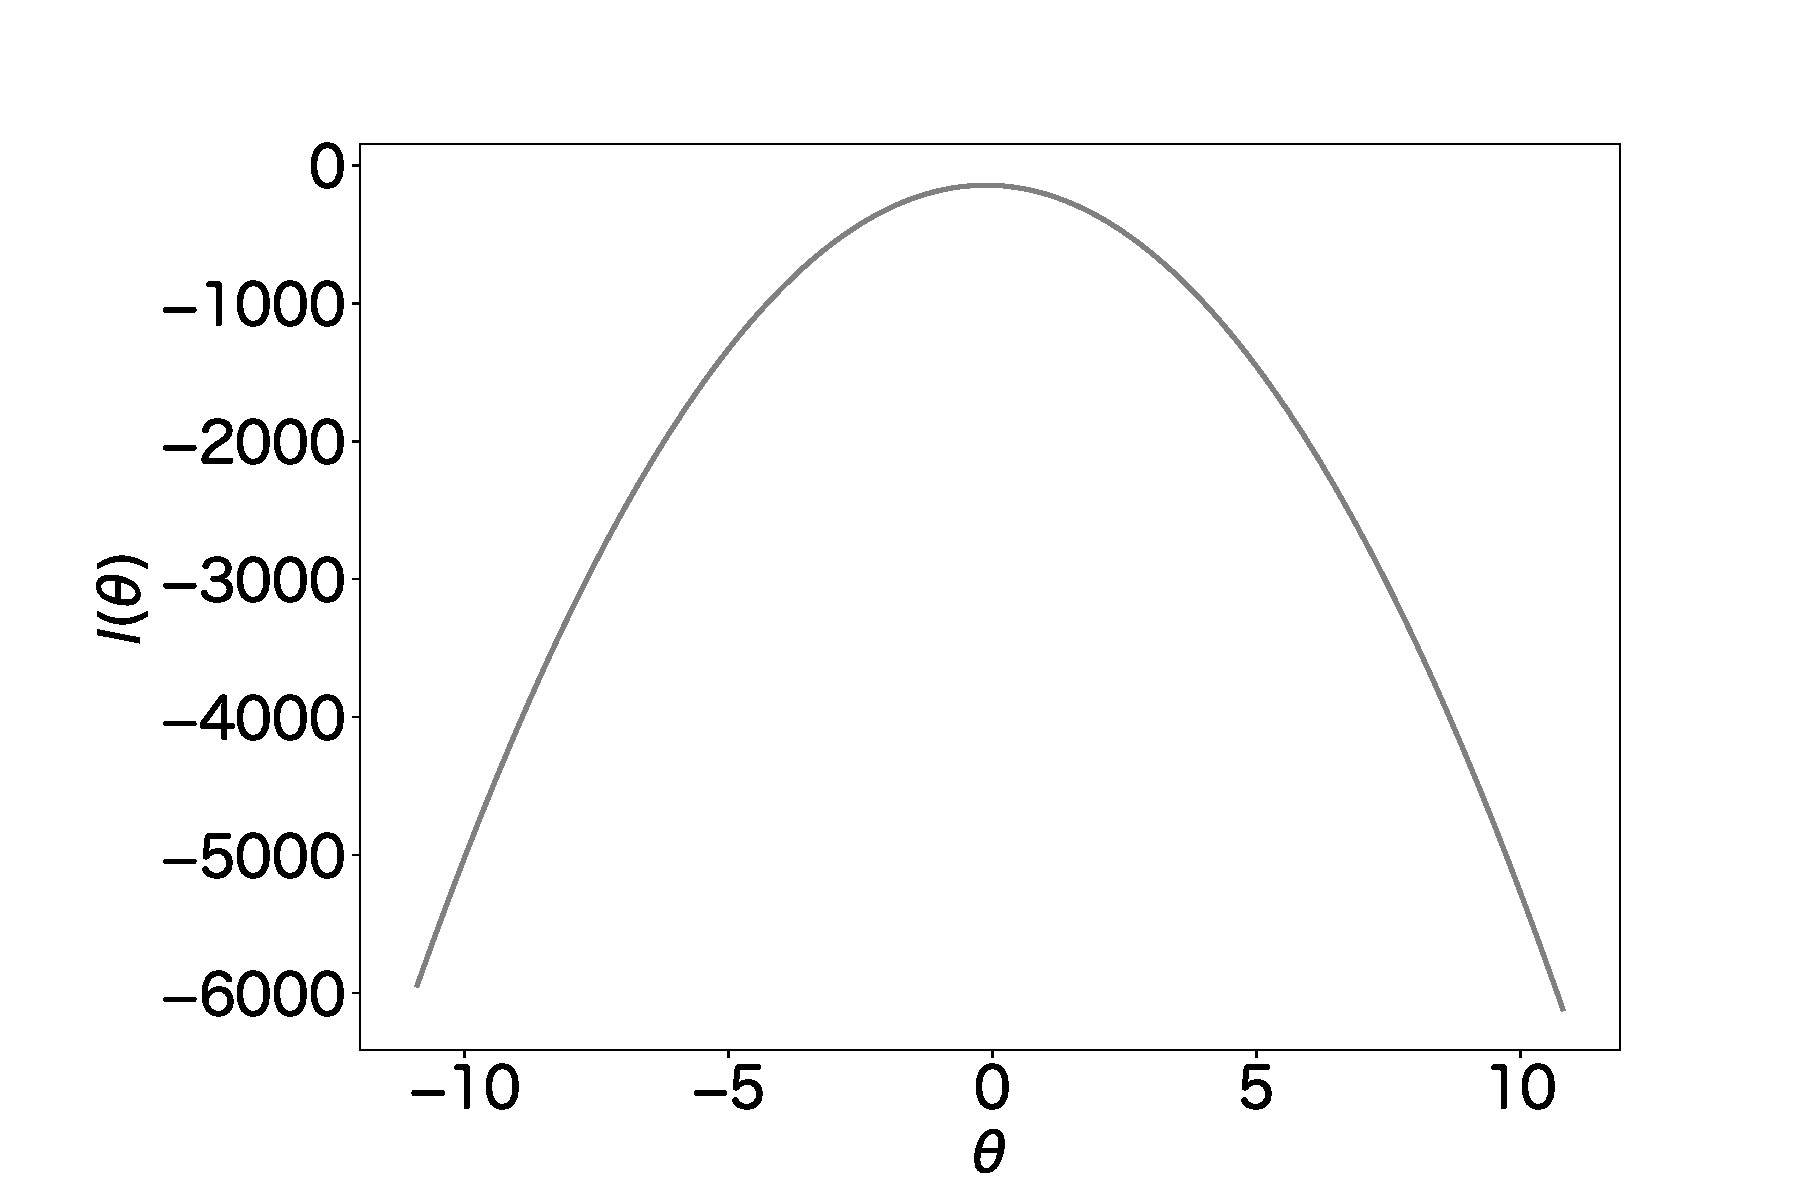
\includegraphics[width=15cm]{./image/02_/loglikelihood_function.pdf}
    \caption{$N(\theta,1)$における対数尤度関数。確率変数は、$N(0,1)$からサンプリングした。}
    \label{fig:loglikelihood_function}
\end{figure}

\subsection{最尤推定}
\begin{defi}
    尤度関数$l(\theta)$を最大にする$\theta$を最尤推定量という。
\end{defi}
正規分布における最尤推定量を計算してみる。正規分布は、母数を二つ持つので、尤度関数も2変数関数である。
まず、対数尤度関数は、
\begin{equation*}
    l(\mu,\sigma^2) = -\frac{n}{2}\log(2\pi\sigma^2)-\frac{1}{2\sigma^2}\sum_{i=1}^n(x_i-\mu)^2 
\end{equation*}
$l(\mu,\sigma^2)$を$\mu$で微分する。
\begin{equation*}
    \frac{\partial l(\mu,\sigma^2)}{\partial \mu} = \frac{\sum_i(x_i-\mu)}{\sigma^2}
\end{equation*}
$\frac{\partial l(\mu,\sigma^2)}{\partial \mu} = 0$とおいて、$\mu$について解くと、
\begin{equation*}
    \mu_{ML} = \frac{\sum_i x_i}{n}
\end{equation*}
これが最尤推定量となる\footnote{最尤がmaximum likelihoodなので頭文字を取ったMLを$\mu$の足に書いて$\mu_{ML}とした$}。
%言い換えれば、最尤推定量

同様に$\sigma^2$に関する微分を行う。
\begin{equation*}
    \frac{\partial l(\mu,\sigma^2)}{\partial \sigma^2} = -\frac{n}{2\sigma^2}+\frac{1}{2\sigma^4}\sum_i(x_i-\mu)
\end{equation*}
これが$0$と等しいとき、$\sigma^2$について解く。
\begin{equation*}
    \sigma^2_{ML} = \frac{\sum_i(x_i-\mu)^2}{n}
\end{equation*}

最尤推定量は、分布関数によって異なるので、計算してみるとよい。

\subsection{AIC(an information criterion)}
確率分布から対数尤度を求め、対数尤度の低い確率分布は、その中で相対的にデータに対して当てはまりの良い確率分布であると考えることができる。
最尤推定量を使った確率分布関数は、データを使って分布関数を決定しているので、データを使わずに求めた分布よりも、データに対して良い分布関数になりがちである。
そこで、対数尤度に対して罰則項を加えたAICを使って、データに対する当てはまりの良さを計算することがある。
\begin{equation*}
    AIC = -2\log f(x|\theta)+2k
\end{equation*}
ここで、$k$はデータによって決まったパラメータの個数である。

